\begin{frame}
    \vspace*{1.2in}
    \begin{center}
        \Large \textbf{Introduction}: Motivation and Background
    \end{center}
\end{frame}

\begin{frame}{{\small We would like to simulate a \textbf{hypersonic system},}}
    \footnotesize
    \begin{columns}
        \begin{column}{0.6\linewidth}
            \centering
            \only<2>{
                \begin{figure}
                    \centering
                    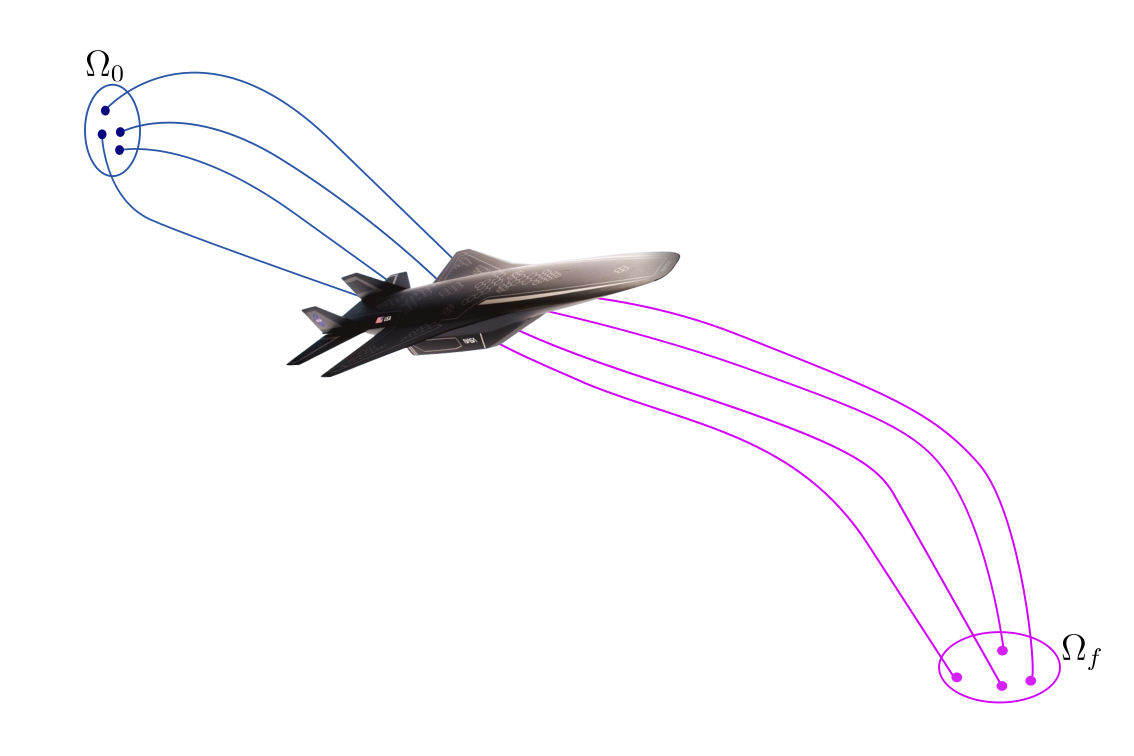
\includegraphics[width=0.9\textwidth]{../figs/introduction/motivating_example_1.png}
                \end{figure}}
            \only<3>{
                \begin{figure}
                    \centering
                    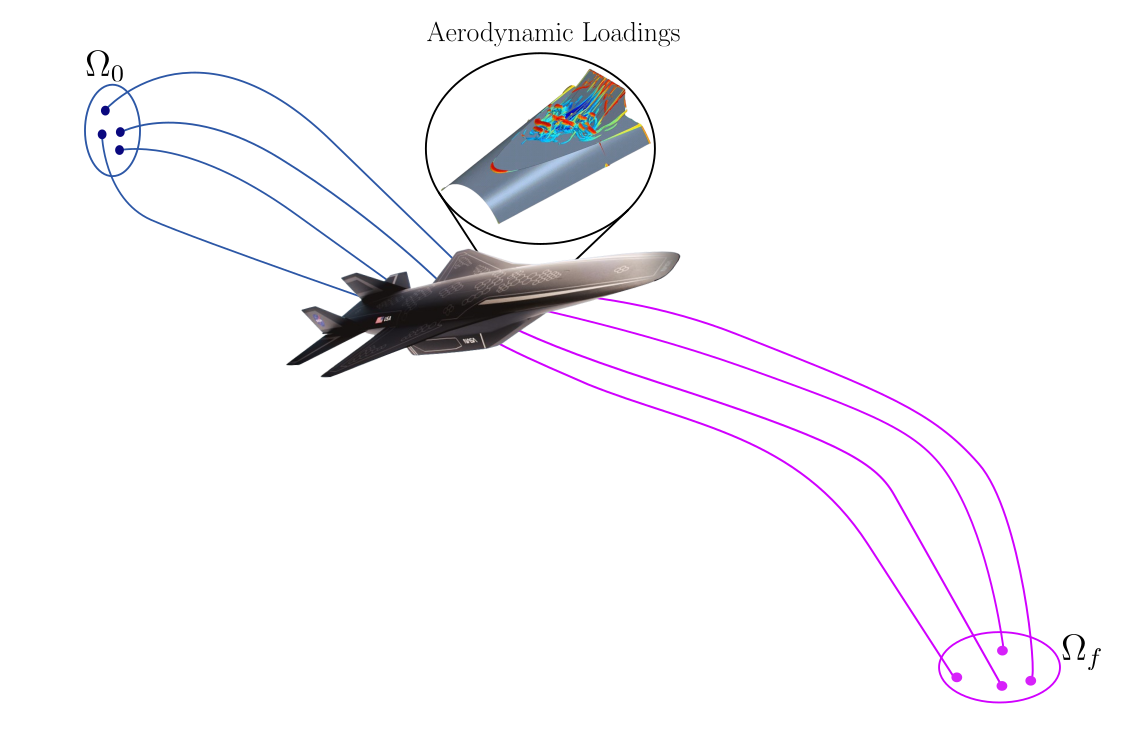
\includegraphics[width=0.9\textwidth]{../figs/introduction/motivating_example_2.png}
                \end{figure}}
            \only<4>{
                \begin{figure}
                    \centering
                    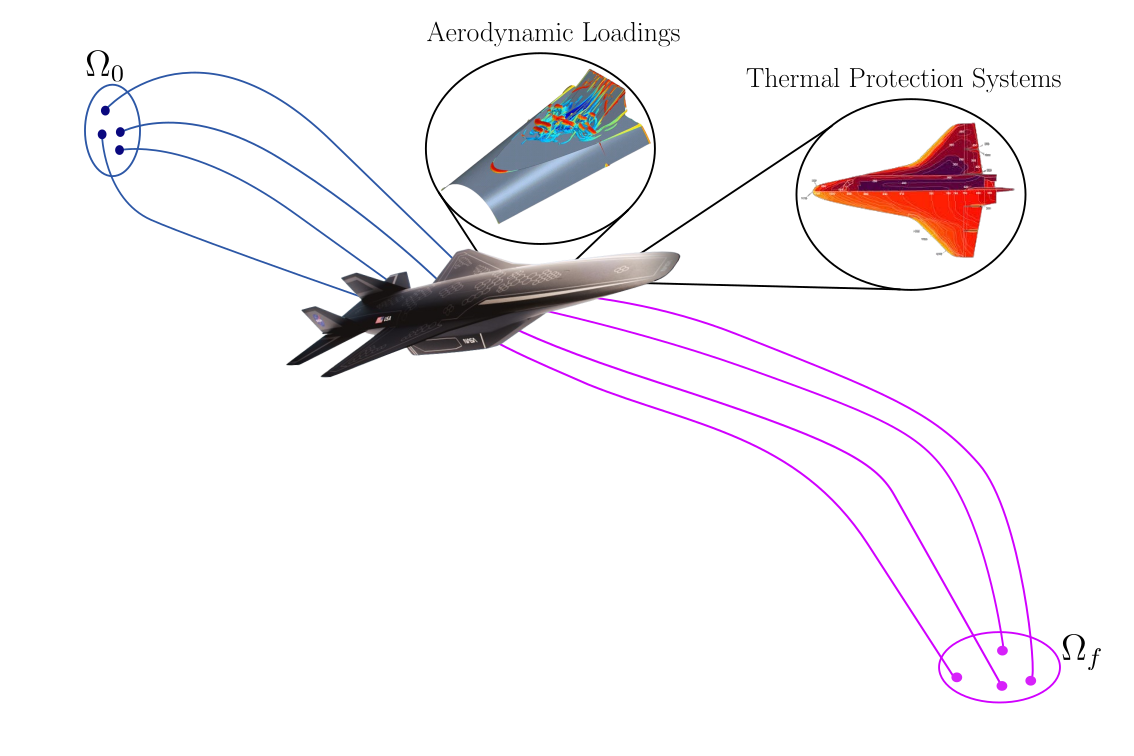
\includegraphics[width=0.9\textwidth]{../figs/introduction/motivating_example_3.png}
                \end{figure}}
            \only<5>{
                \begin{figure}
                    \centering
                    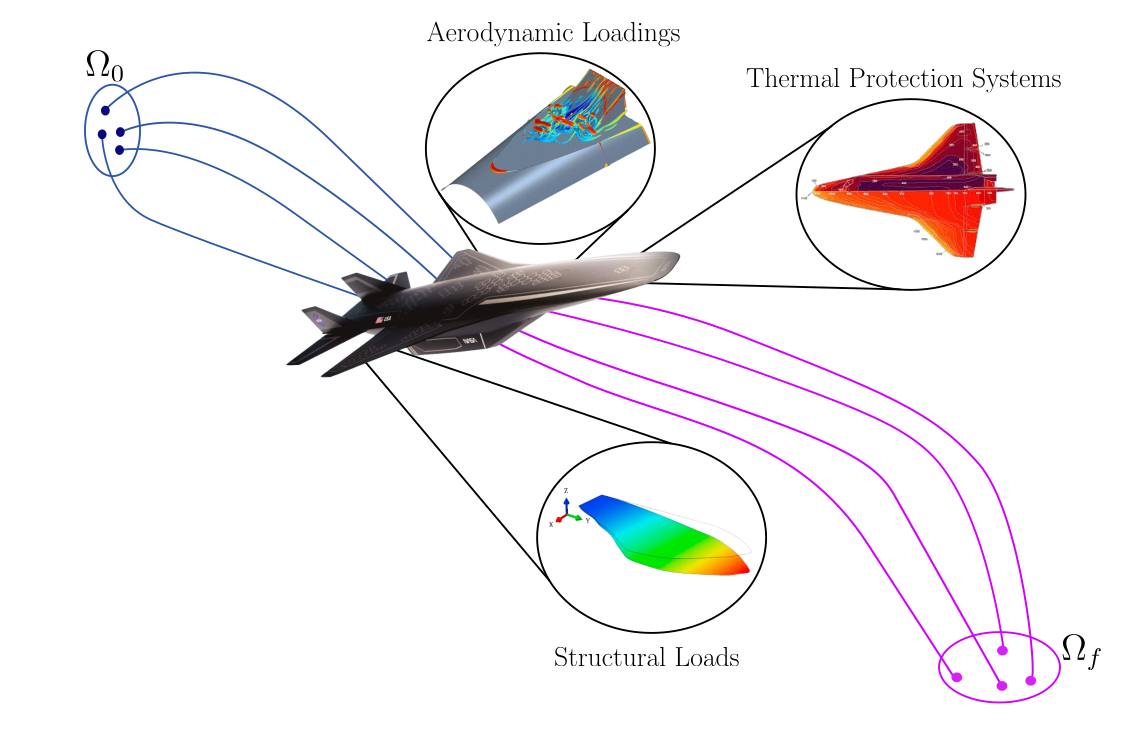
\includegraphics[width=0.9\textwidth]{../figs/introduction/motivating_example_4.png}
                \end{figure}}
            \only<6->{
                \begin{figure}
                    \centering
                    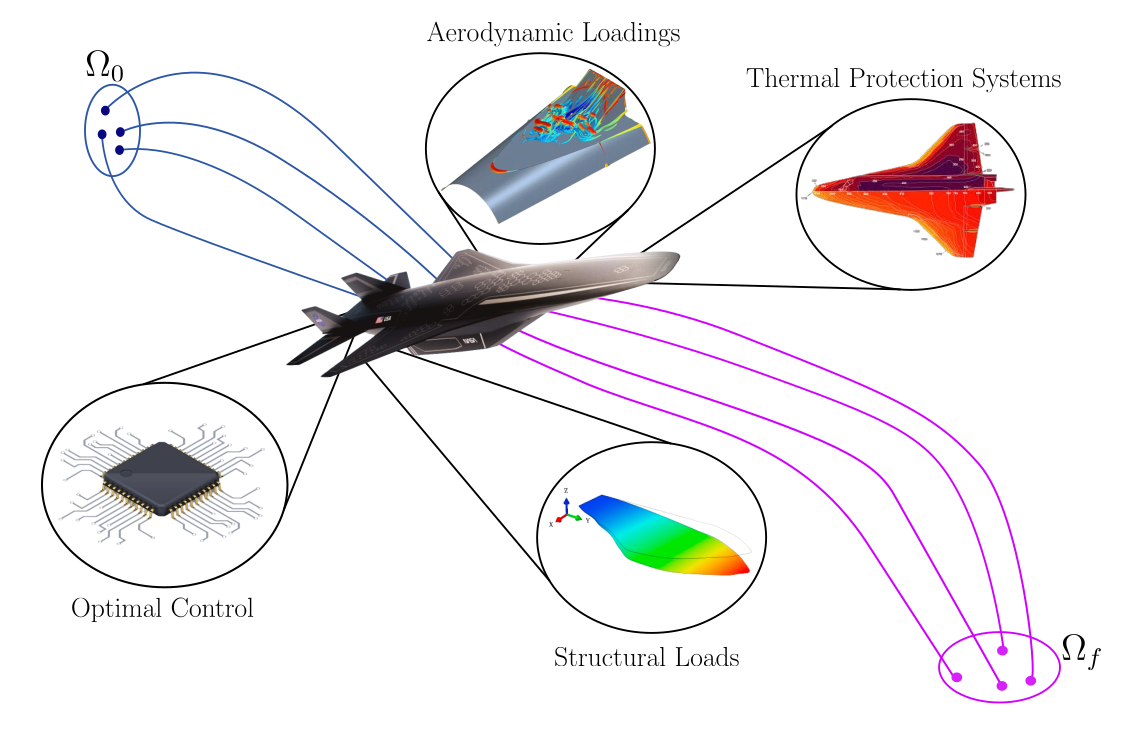
\includegraphics[width=0.9\textwidth]{../figs/introduction/motivating_example_5.png}
                \end{figure}}
        \end{column}
        \hspace*{-1in}
        \begin{column}{0.49\linewidth}
            \centering
            \visible<7-10>{
            \textbf{Finite-Element Model (FEM)}
            \begin{align*}
                \visible<8->{
                \dot{\vu} &= \mathbf{F}\left(\vu;\mathbf{p}\right)}\\
                \visible<9->{
                \vz_{\text{HF}} &= \mathbf{H}\left(\vu;\vp\right)}\\
                \visible<10->{
                \vu(t_0) &= \vu_0(\vp)}
            \end{align*}
            }
            \visible<11-14>{
            \textbf{Optimal Control Problem (OCP)}
            \begin{align*}
                \visible<12->{
                \min_{\vp} \: \mathcal{J} = \int_{t_0}^{t_f} & \ell\left(\vu,\mathbf{p}\right) dt}\\
                \visible<13->{
                \text{s.t.} \: \quad \dot{\vu} &= \mathbf{F}\left(\vu;\mathbf{p}\right)}\\
                \visible<14->{
                \mathbf{Q} &\geq \mathbf{g}\left(\vu(t),t;\mathbf{p}\right)}
            \end{align*}
            }
        \end{column}
    \end{columns}
    \visible<2->{
    \begin{center}
        {\tiny
        $\vu$: high-dimensional states, $\vF$: non-linear dynamics $\vp$: design/control parameters, $\vz_{\text{HF}}$: high-fidelity outputs, $\mathcal{J}$: cost functional, $l$: running cost, $\mathbf{Q}$: safety bound, $\vg$: constraint function}
    \end{center}}
\end{frame}

\begin{frame}{{\small \textbf{High-Fidelity} exploration of design space is costly,}}
    \footnotesize
    \vspace*{-0.1in}
    \only<1>{
        \begin{figure}
            \centering
            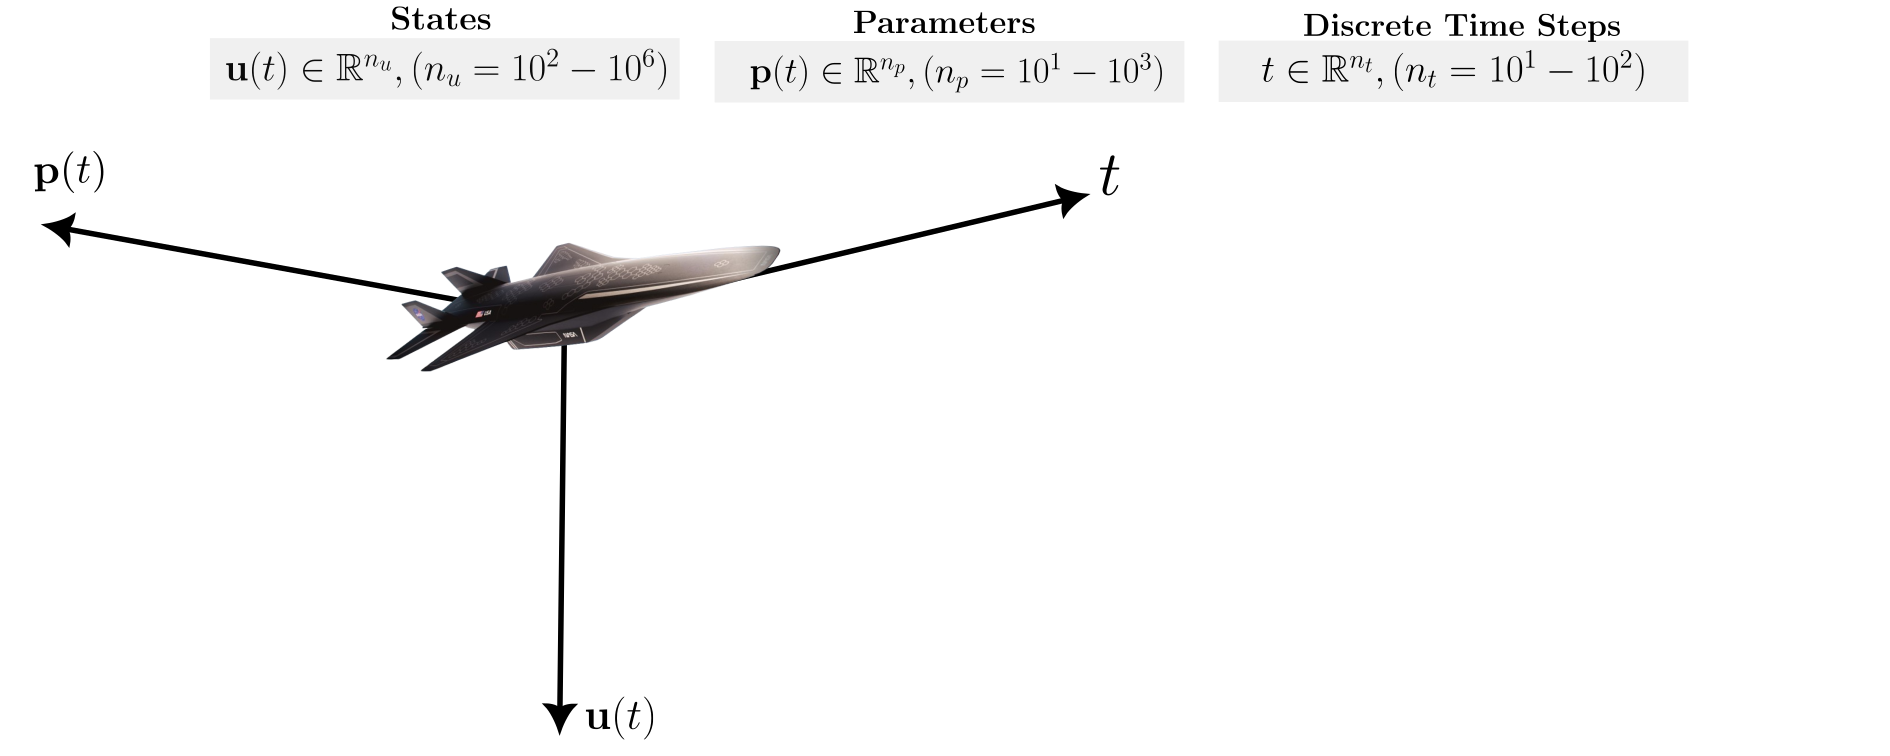
\includegraphics[width=0.95\textwidth]{../figs/introduction/problem_space_1.png}
        \end{figure}}
    \only<2>{
        \begin{figure}
            \centering
            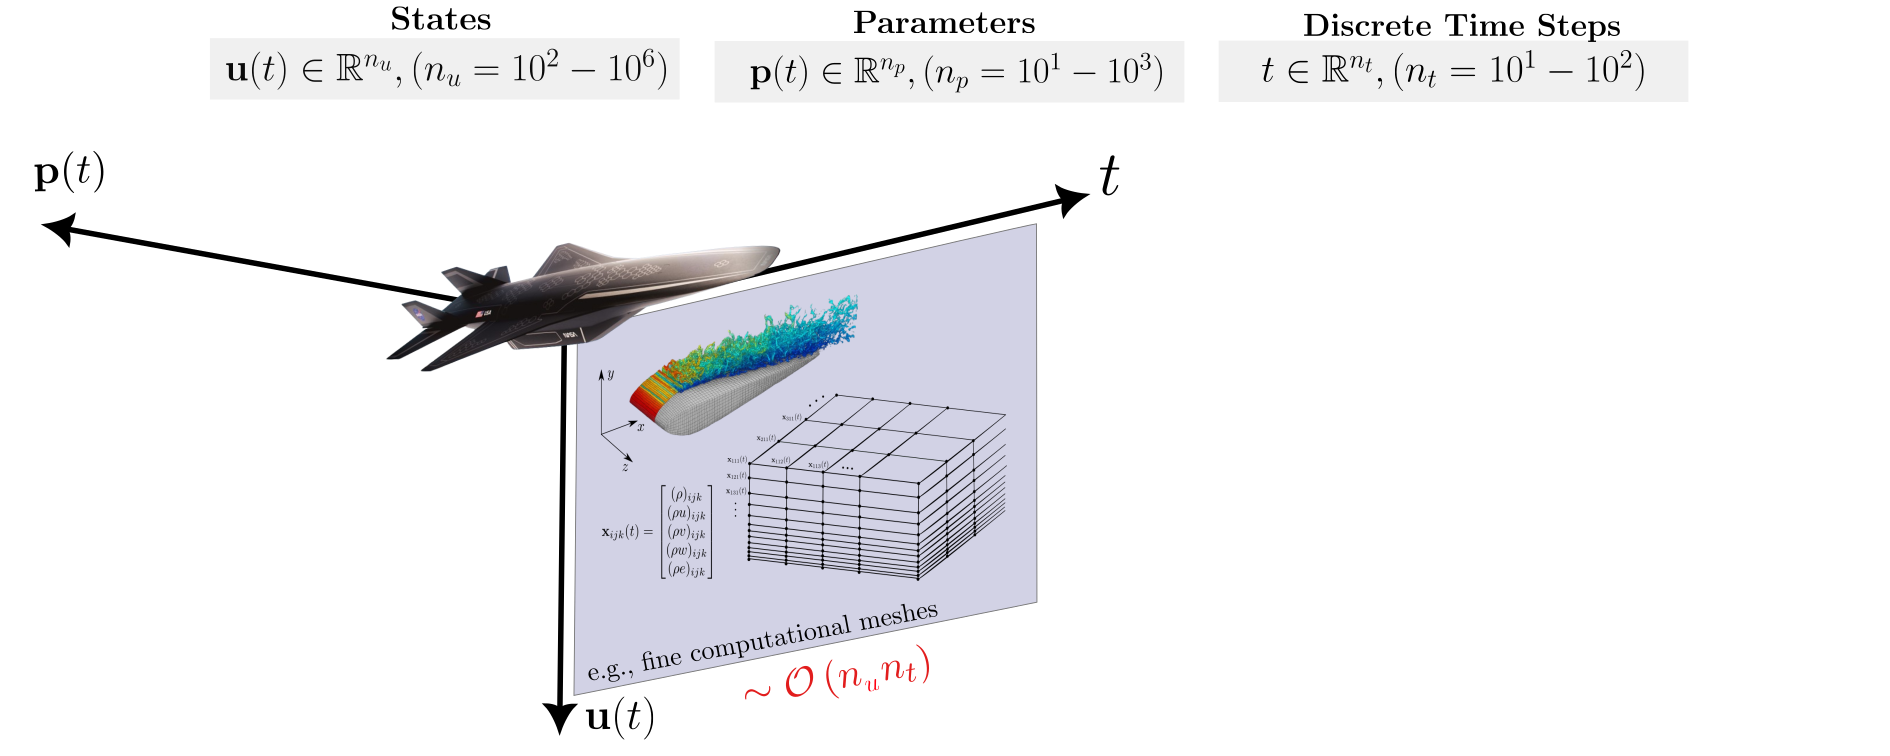
\includegraphics[width=0.95\textwidth]{../figs/introduction/problem_space_2.png}
        \end{figure}}
    \only<3>{
        \begin{figure}
            \centering
            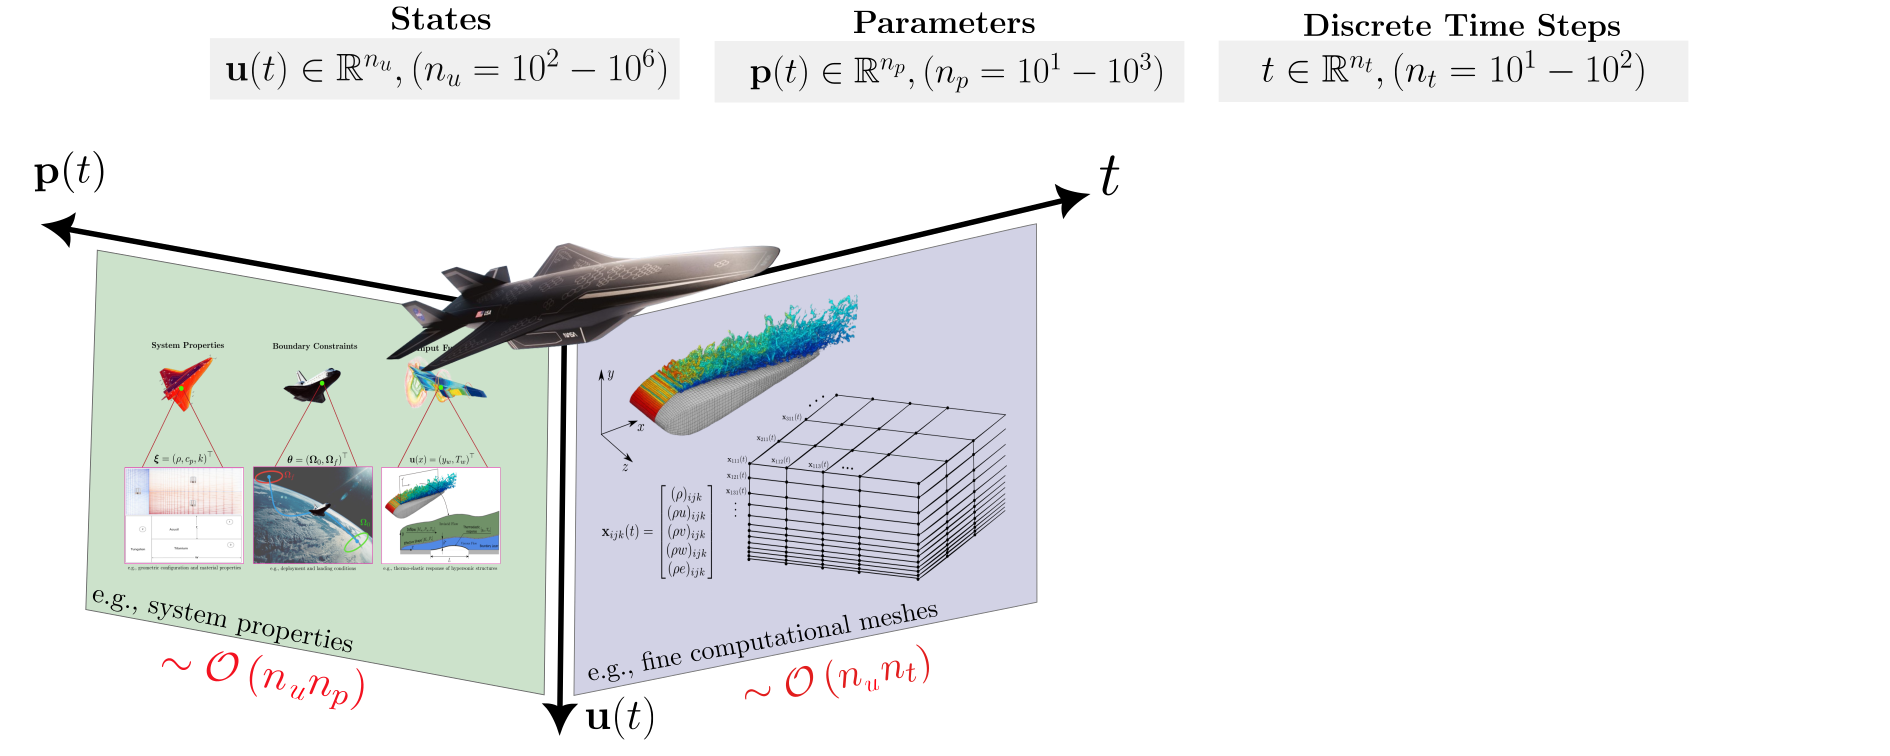
\includegraphics[width=0.95\textwidth]{../figs/introduction/problem_space_3.png}
        \end{figure}}
    \only<4>{
        \begin{figure}
            \centering
            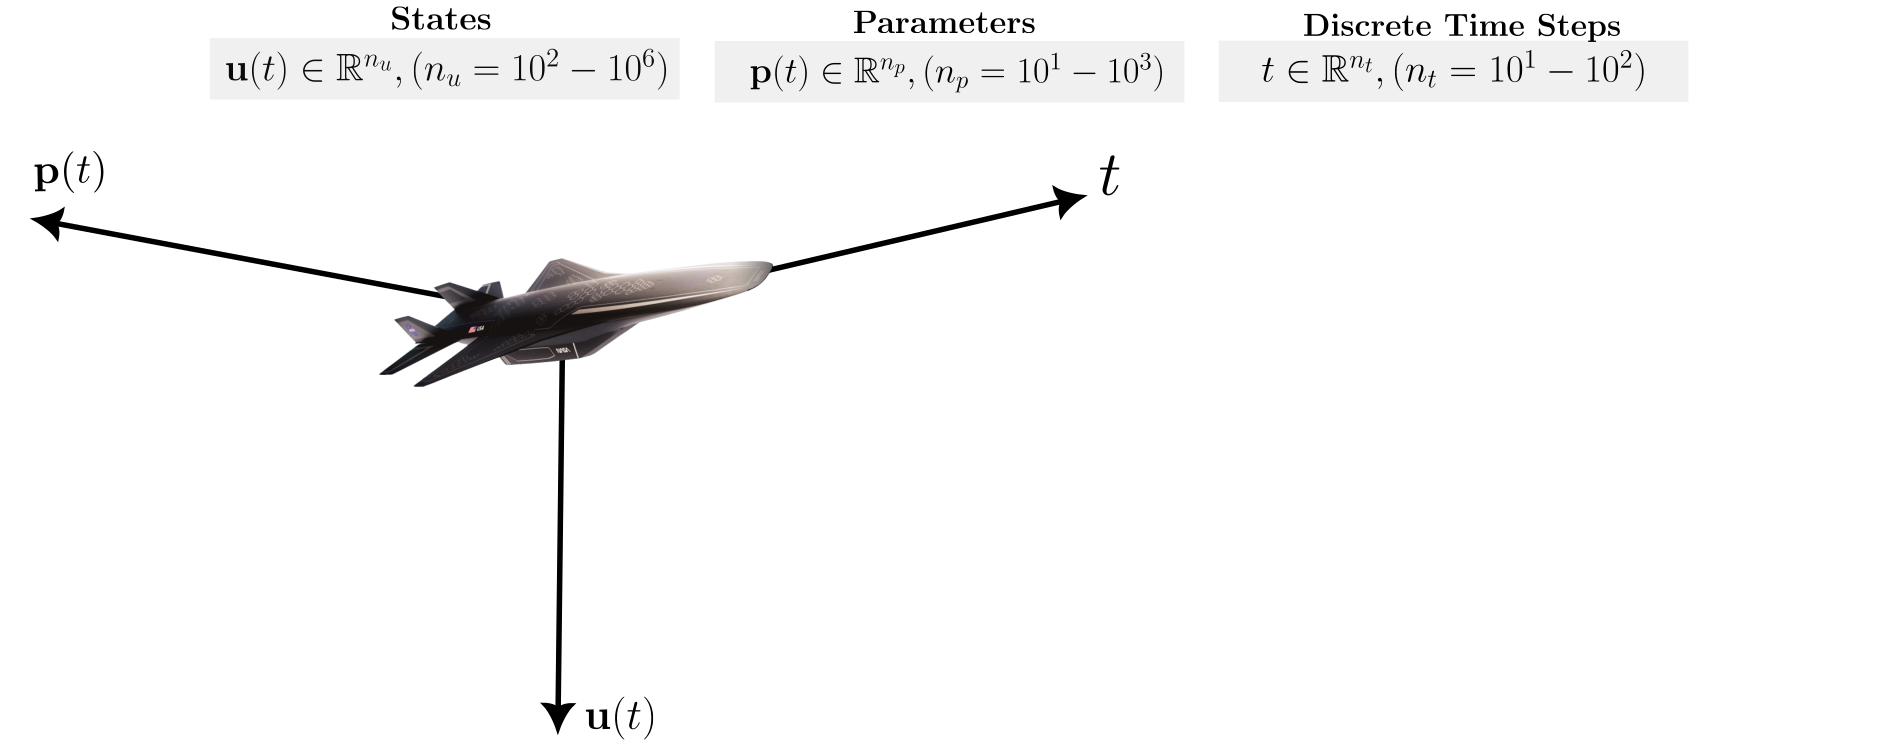
\includegraphics[width=0.95\textwidth]{../figs/introduction/problem_space_4.png}
        \end{figure}}
    \only<5>{
        \begin{figure}
            \centering
            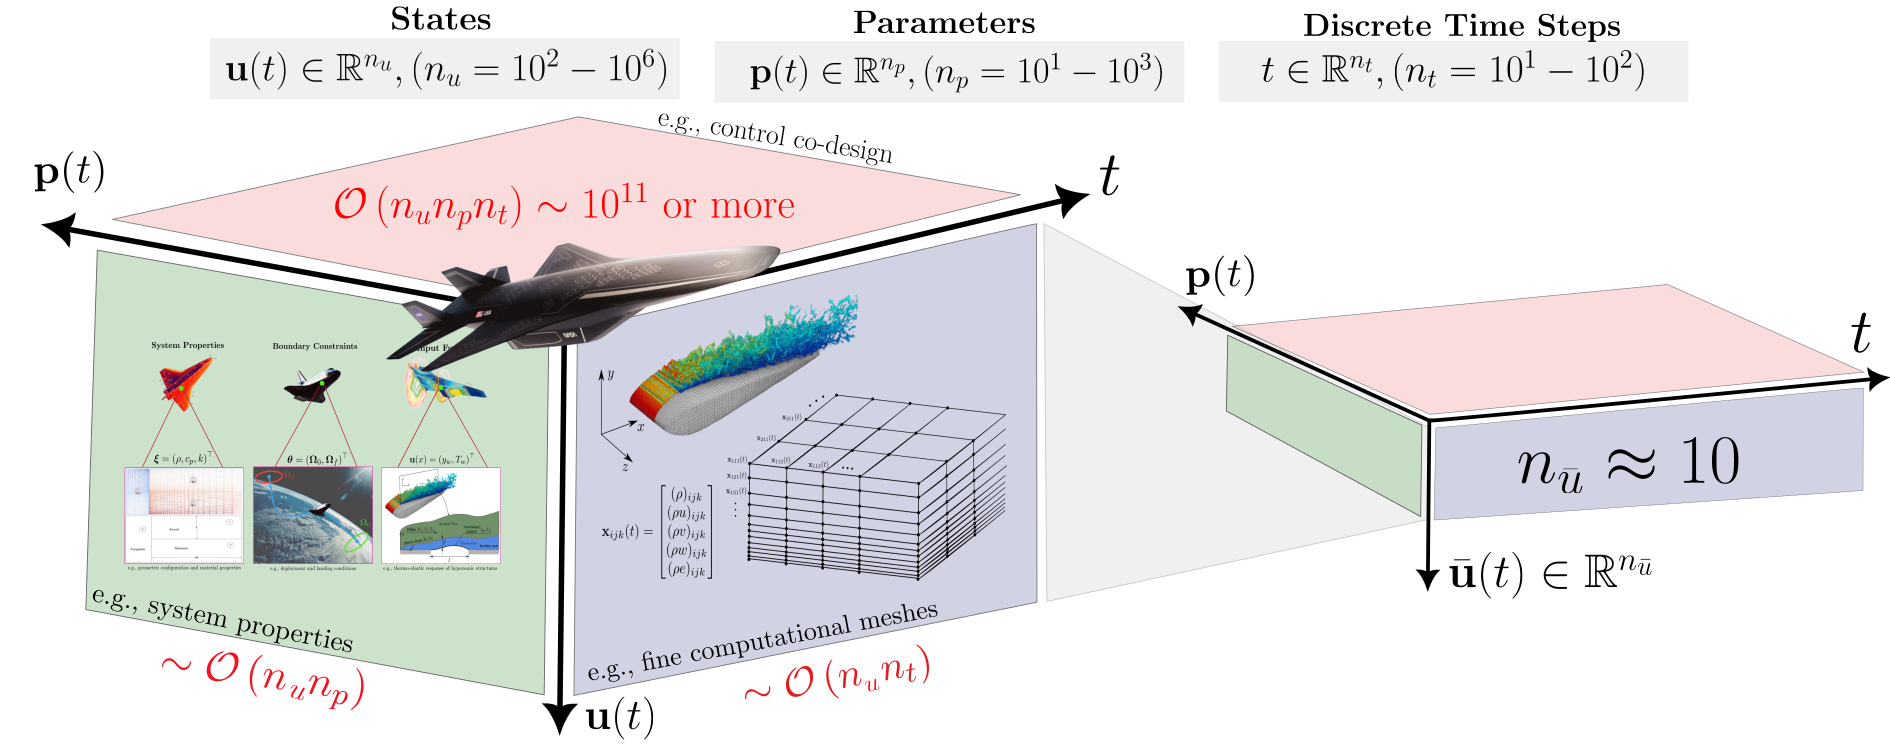
\includegraphics[width=0.95\textwidth]{../figs/introduction/problem_space_5.png}
        \end{figure}}
    \only<6>{
        \begin{figure}
            \centering
            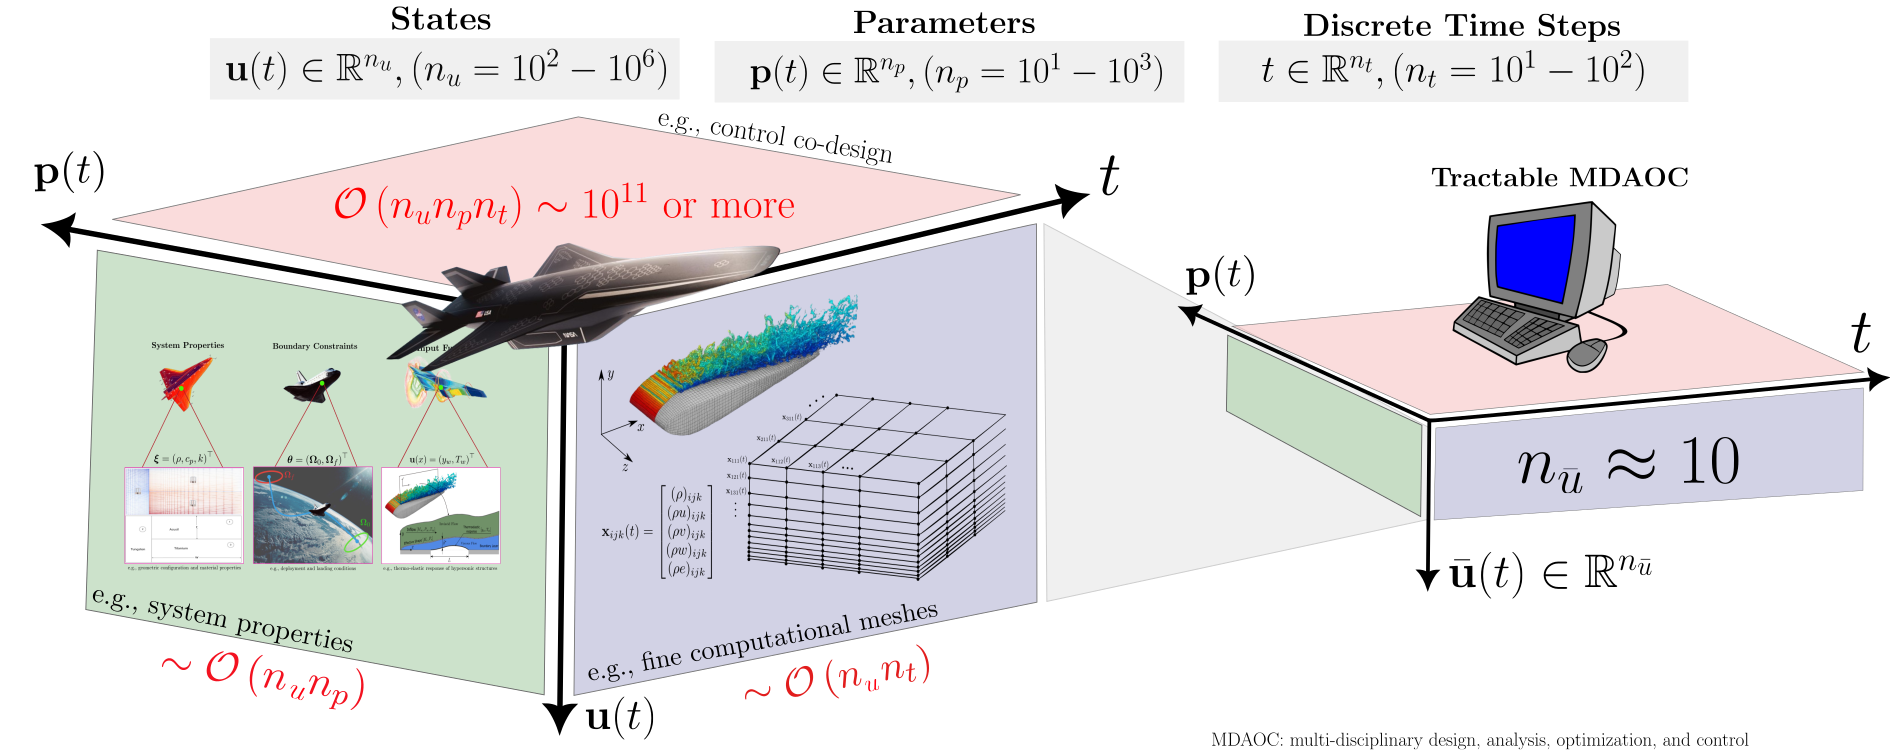
\includegraphics[width=0.95\textwidth]{../figs/introduction/problem_space_6.png}
        \end{figure}}
    \only<7->{
        \begin{figure}
            \centering
            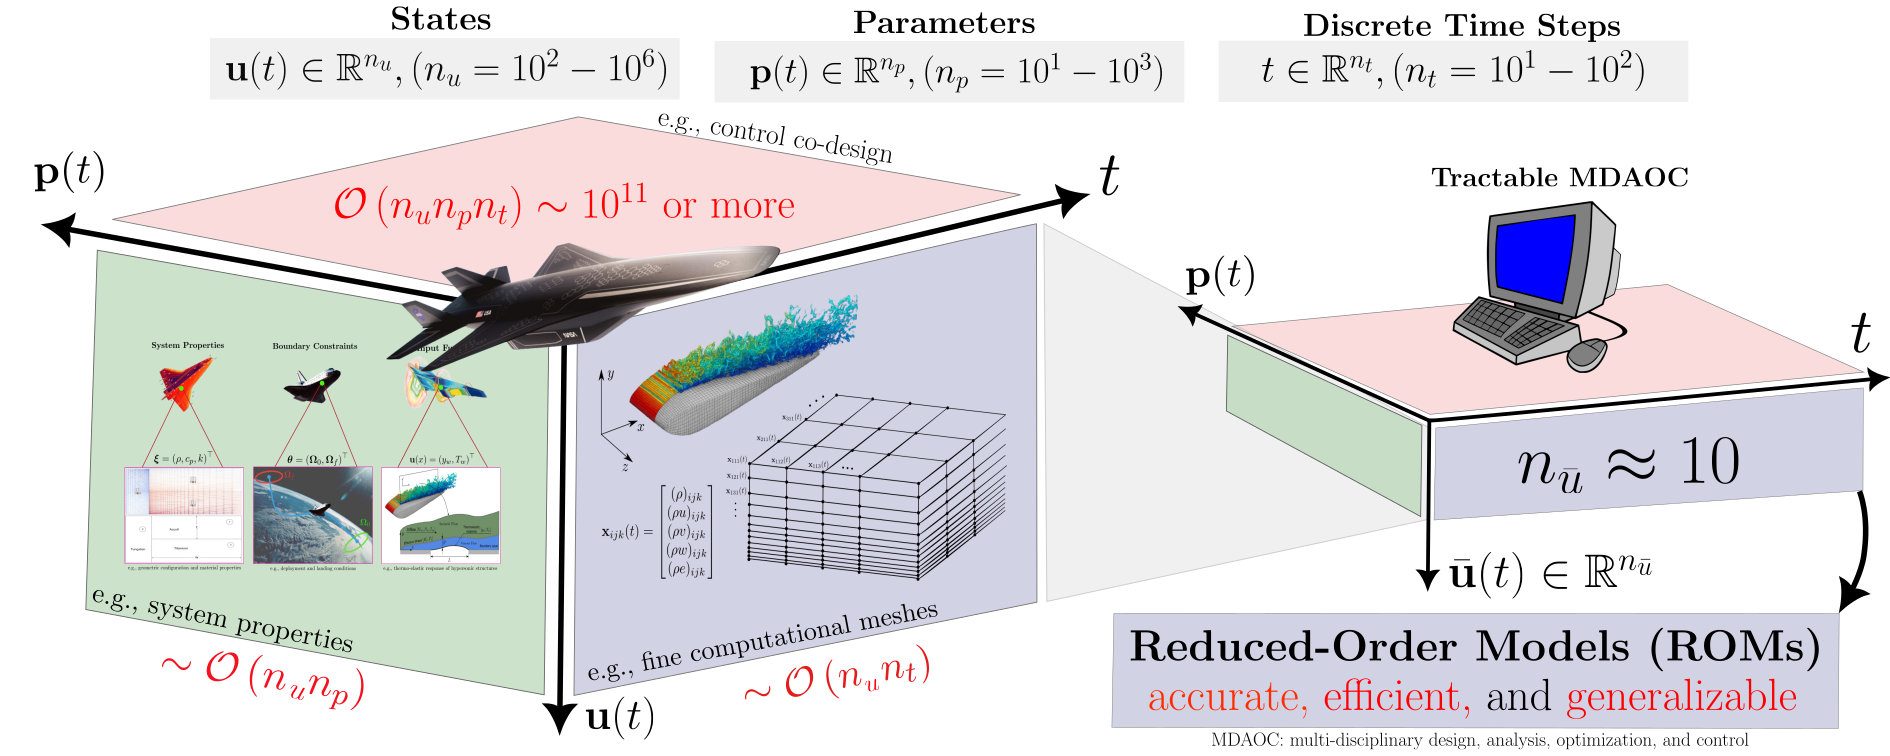
\includegraphics[width=0.95\textwidth]{../figs/introduction/problem_space_7.png}
        \end{figure}}
\end{frame}

\begin{frame}{{\small Balance \textbf{Accuracy}, \textbf{Efficiency}, and \textbf{Generalizability}},}
    \footnotesize
    \begin{columns}
        \begin{column}{0.65\textwidth}
            \centering
            \only<1-2>{
                \begin{figure}
                    \centering
                    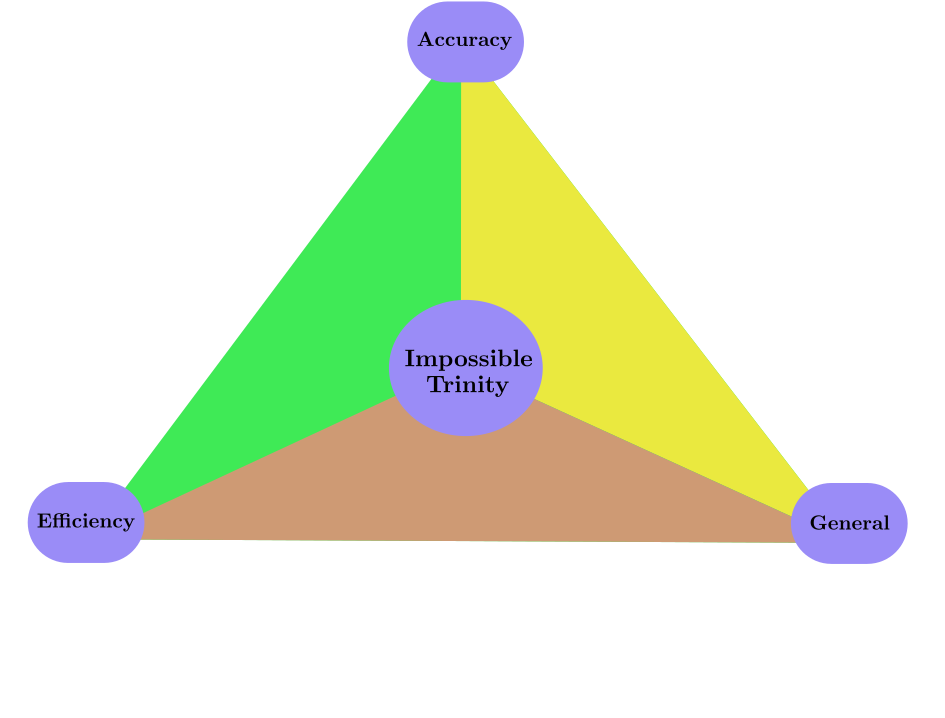
\includegraphics[width=0.8\textwidth]{../figs/introduction/itm_1.png}
                \end{figure}}
            \only<3>{
                \begin{figure}
                    \centering
                    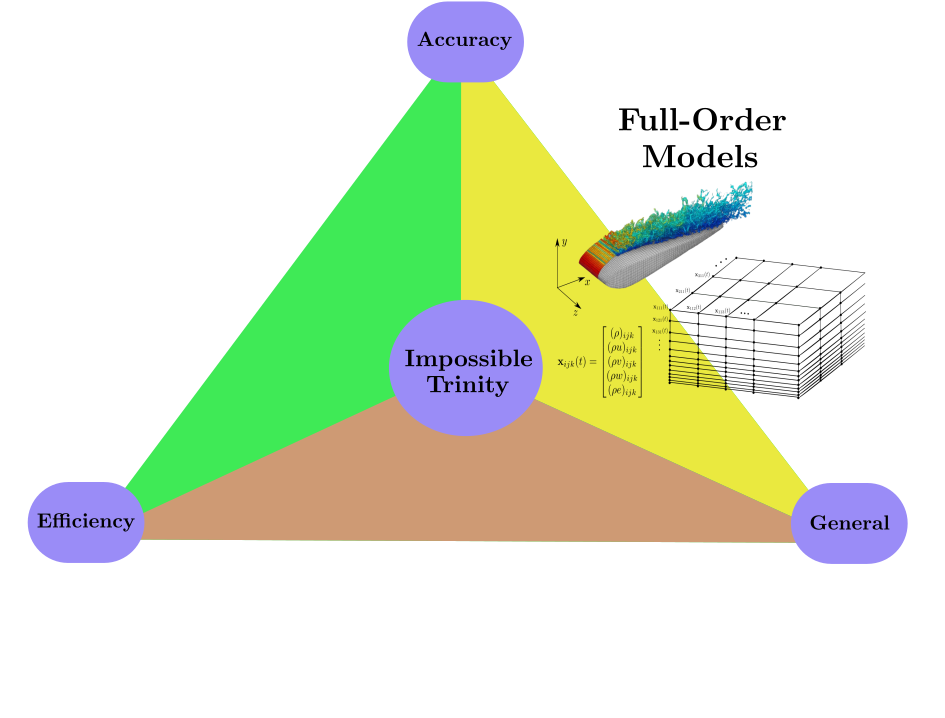
\includegraphics[width=0.8\textwidth]{../figs/introduction/itm_2.png}
                \end{figure}}
            \only<4>{
                \begin{figure}
                    \centering
                    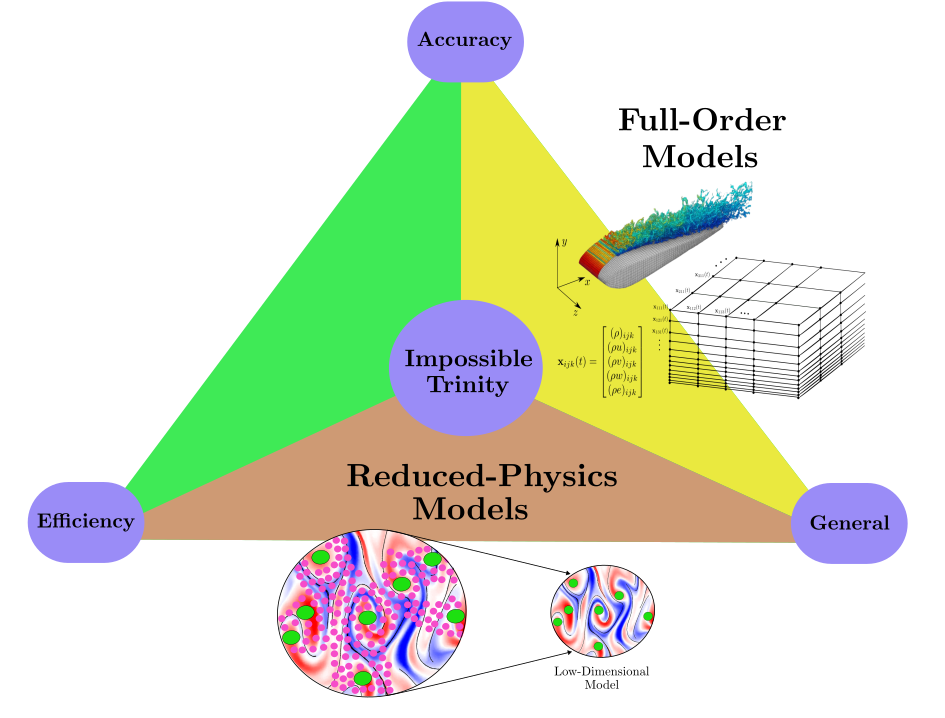
\includegraphics[width=0.8\textwidth]{../figs/introduction/itm_3.png}
                \end{figure}}
            \only<5->{
                \begin{figure}
                    \centering
                    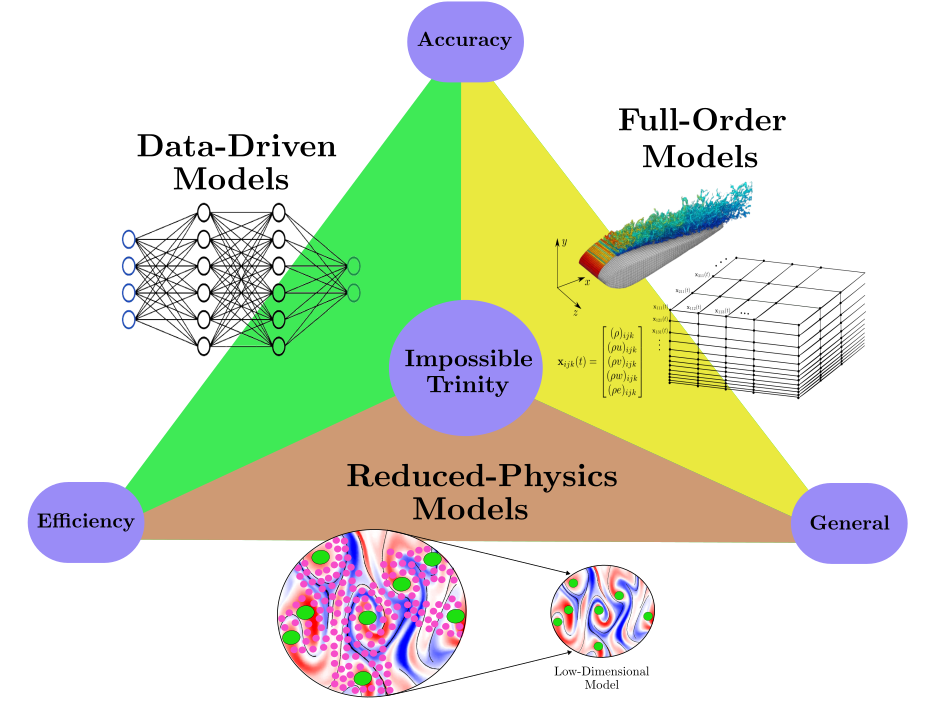
\includegraphics[width=0.8\textwidth]{../figs/introduction/itm_4.png}
                \end{figure}}
            \vspace{-0.3in}
        \end{column}
        \hspace*{-0.7in}
        \begin{column}{0.50\textwidth}
            \vspace*{0.5in}
            \centering
            \visible<2->{
            \begin{center}
                Remains largely \textbf{unresolved} because,
            \end{center}}
            \vspace*{-0.1in}
            \begin{itemize}
                \item<3-> \textbf{FOMs}: too many states,
                \item<4-> \textbf{RPMs}: overly simplified problems,
                \item<5-> \textbf{Data-driven models}: need too much data.
            \end{itemize}
        \end{column}
    \end{columns}
\end{frame}

% % \begin{frame}{\small Persistent issues with \textbf{state-of-the-art} approaches,}
% %     \vspace*{-0.2in}
% %     \footnotesize
% %     \only<1>{
% %     \begin{figure}
% %         \centering
% %         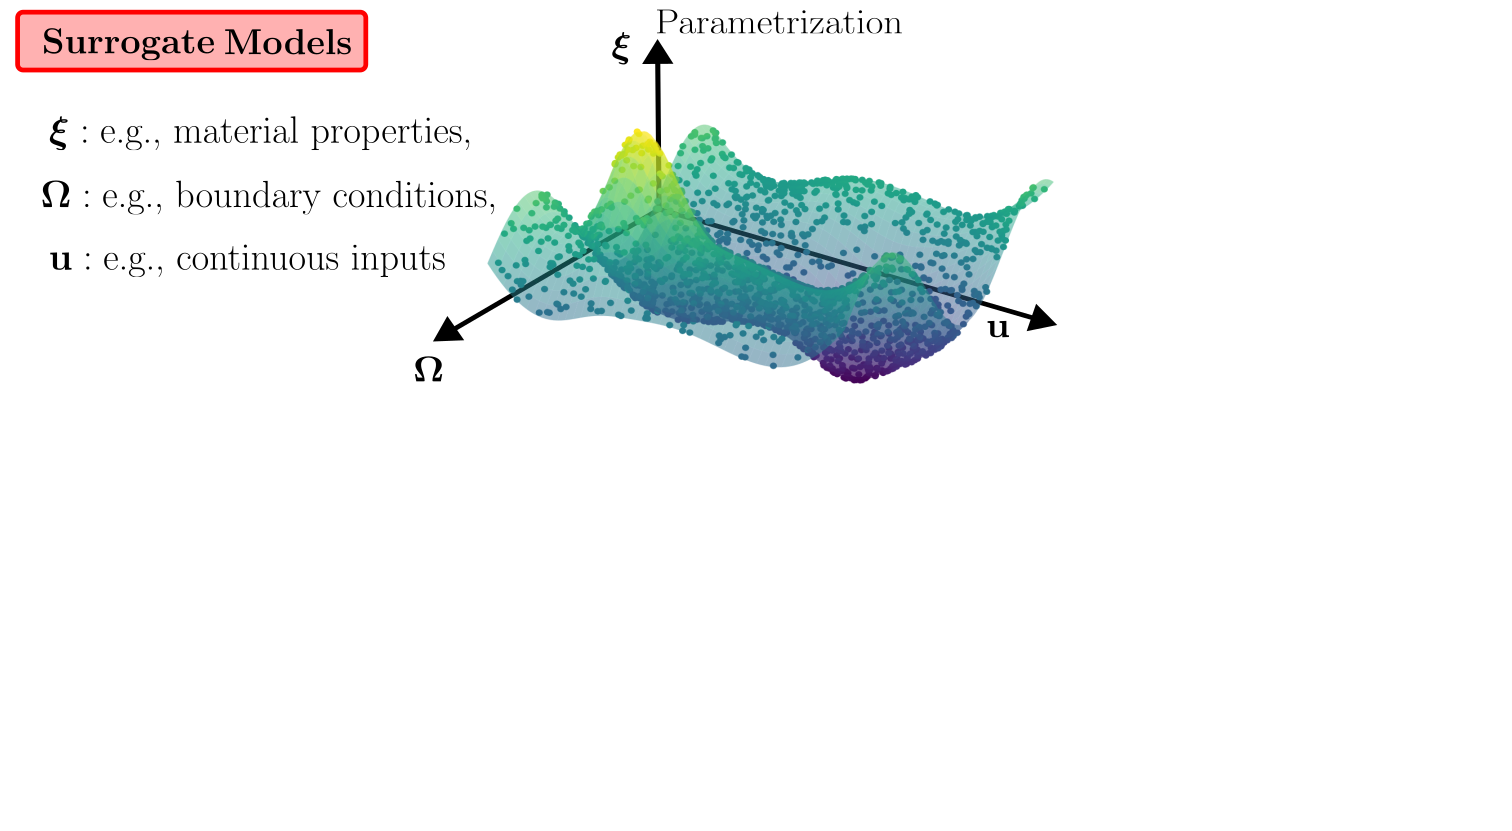
\includegraphics[width=0.9\textwidth]{../figs/sota/surrogates_1.png}
% %     \end{figure}}
% %     \only<2>{
% %     \begin{figure}
% %         \centering
% %         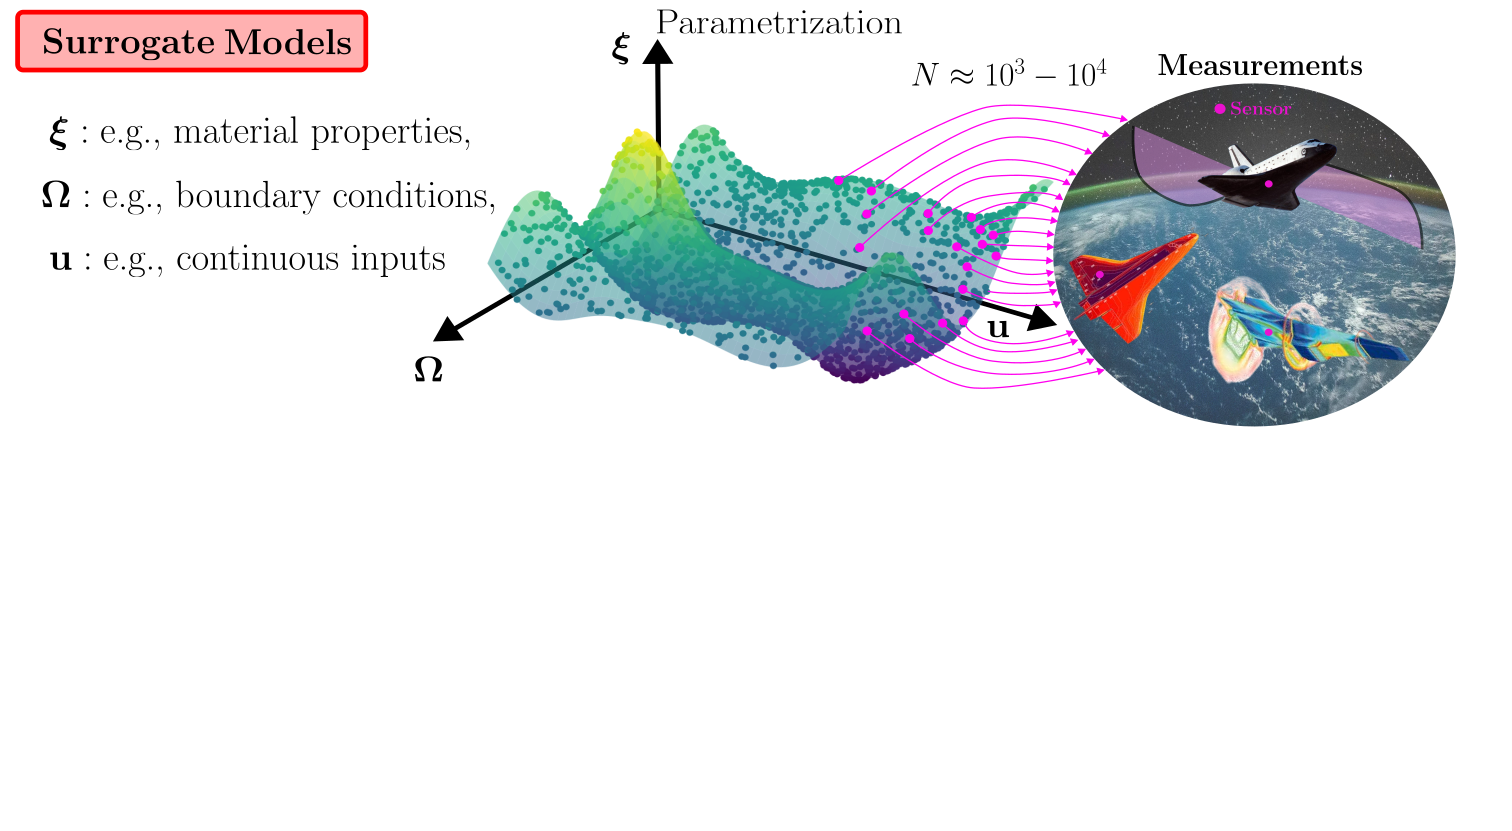
\includegraphics[width=0.9\textwidth]{../figs/sota/surrogates_2.png}
% %     \end{figure}}
% %     \only<3>{
% %     \begin{figure}
% %         \centering
% %         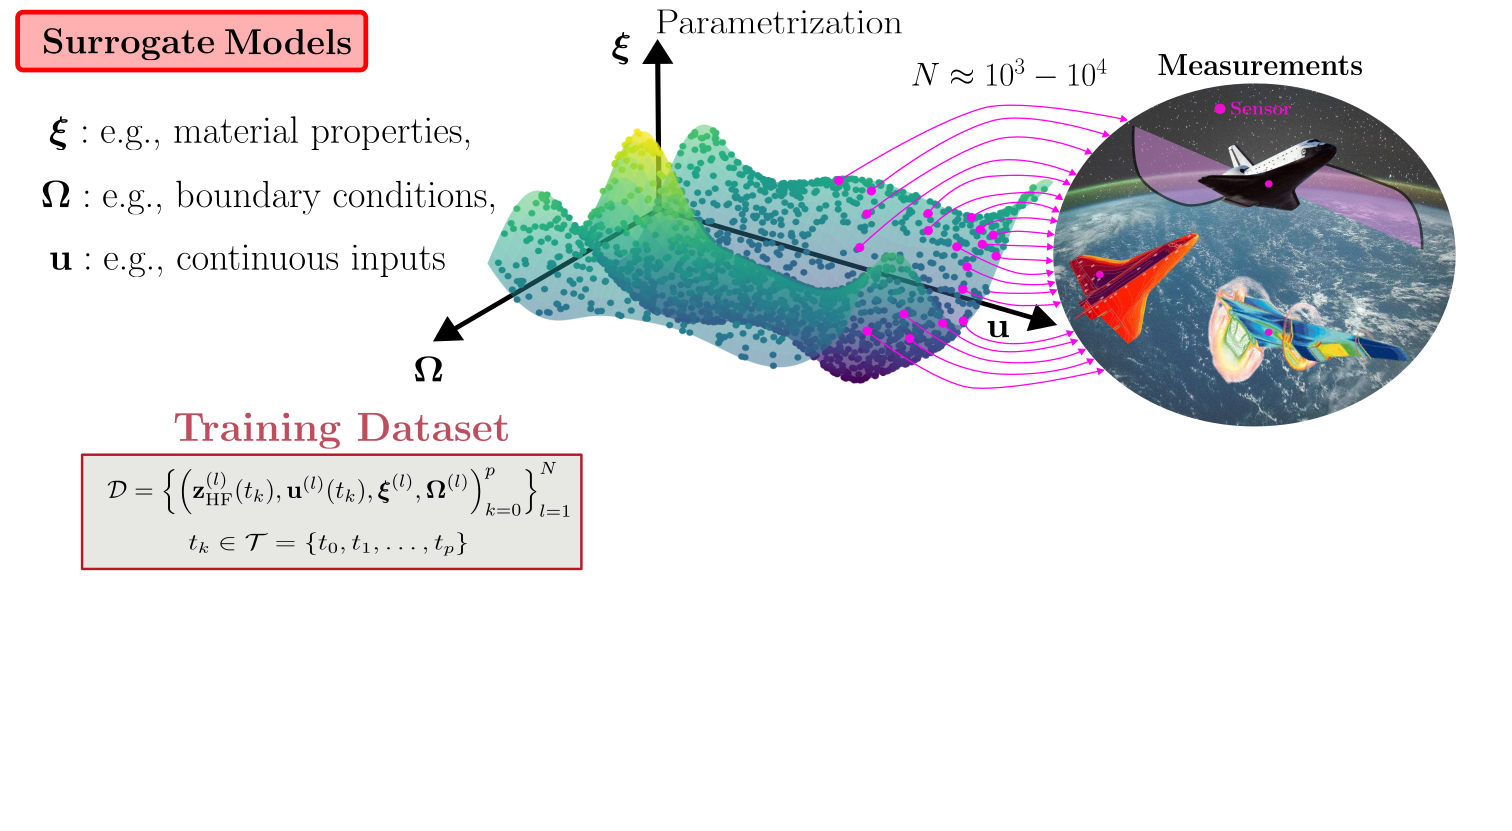
\includegraphics[width=0.9\textwidth]{../figs/sota/surrogates_3.png}
% %     \end{figure}}
% %     \only<4>{
% %     \begin{figure}
% %         \centering
% %         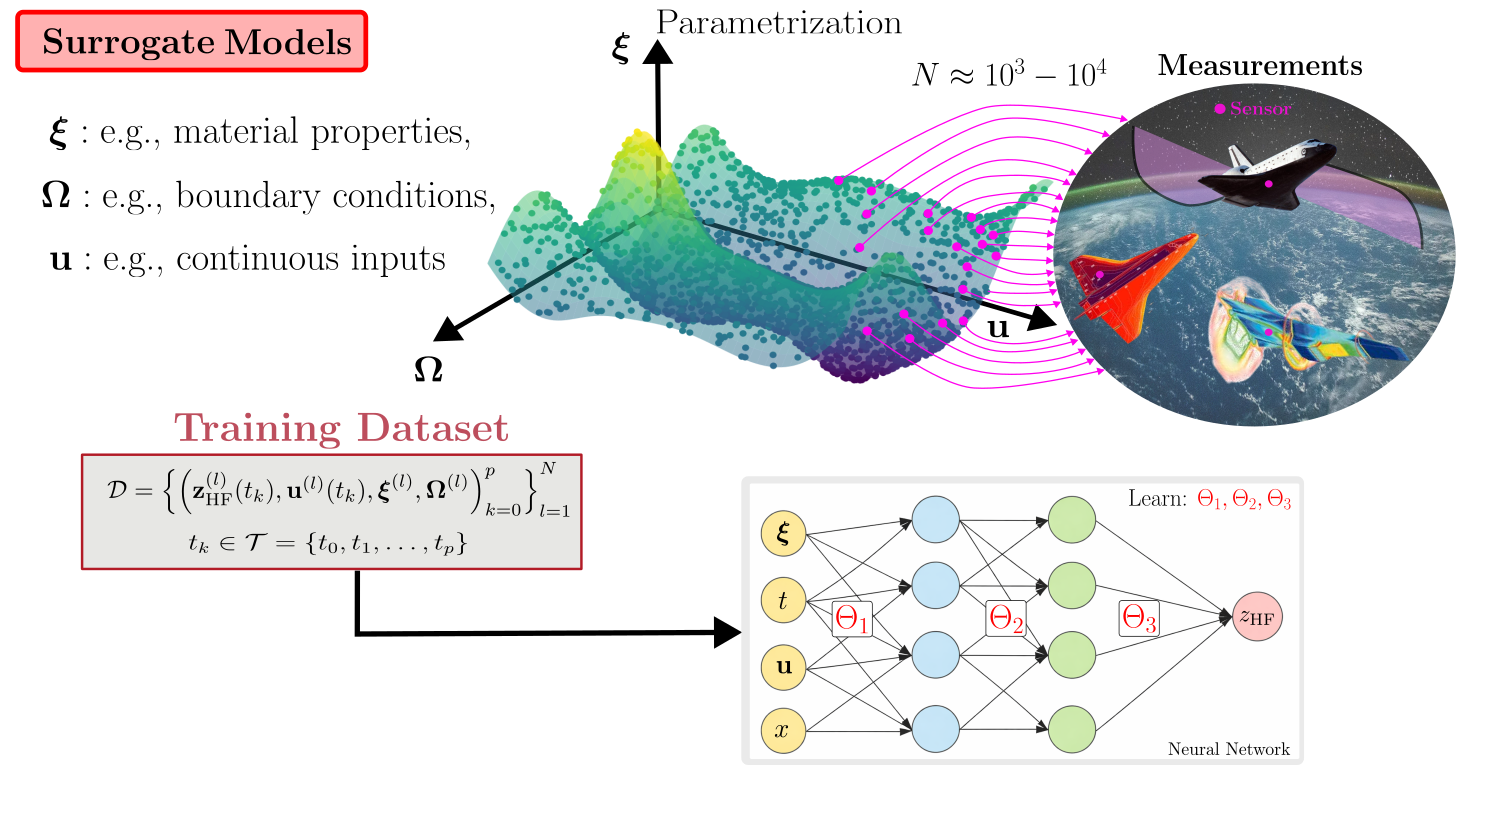
\includegraphics[width=0.9\textwidth]{../figs/sota/surrogates_4.png}
% %     \end{figure}}
% %     \only<5>{
% %     \begin{figure}
% %         \centering
% %         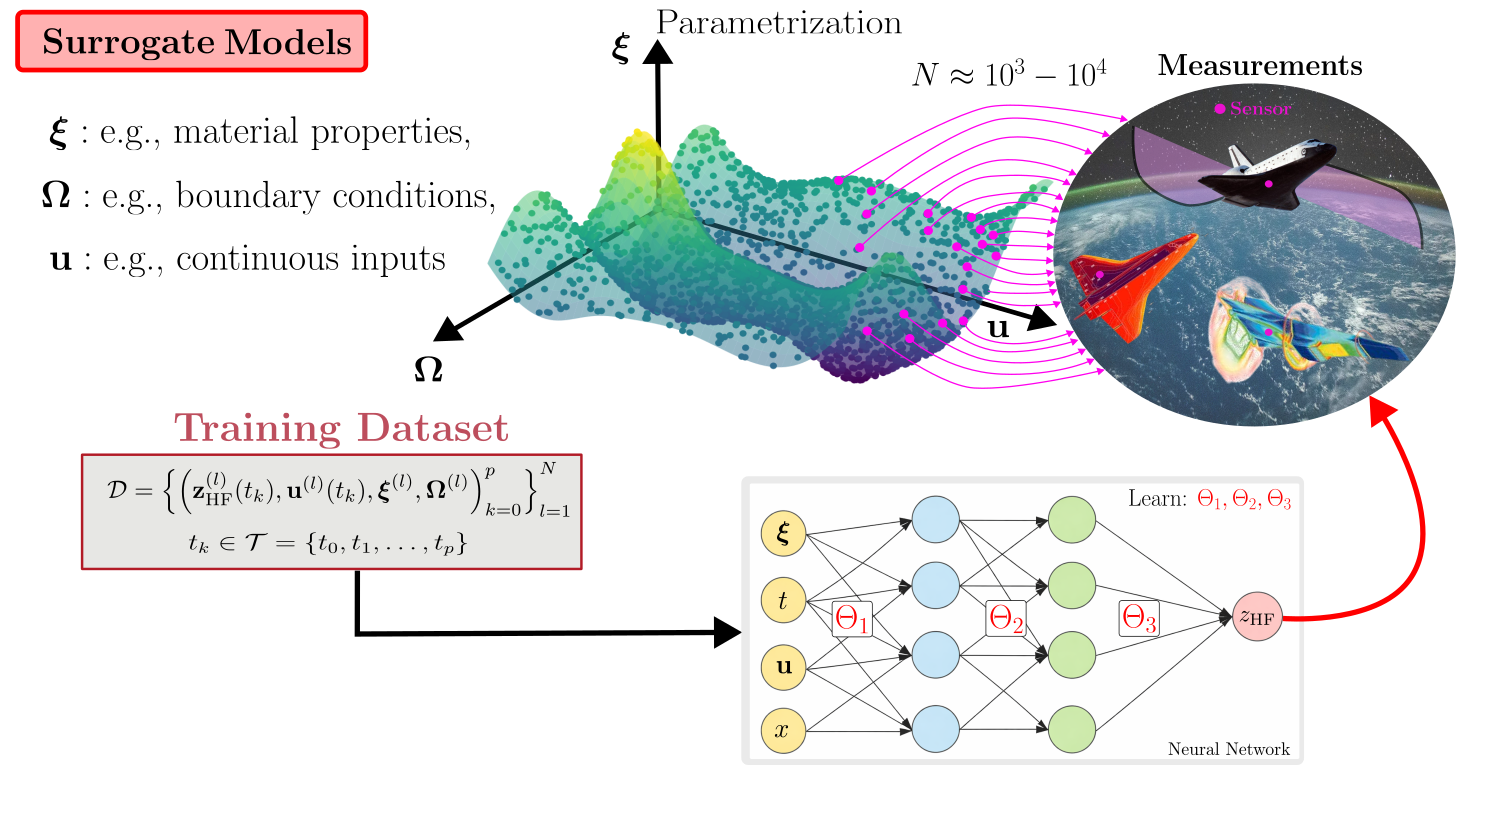
\includegraphics[width=0.9\textwidth]{../figs/sota/surrogates_5.png}
% %     \end{figure}}
% %     \only<6>{
% %     \begin{figure}
% %         \centering
% %         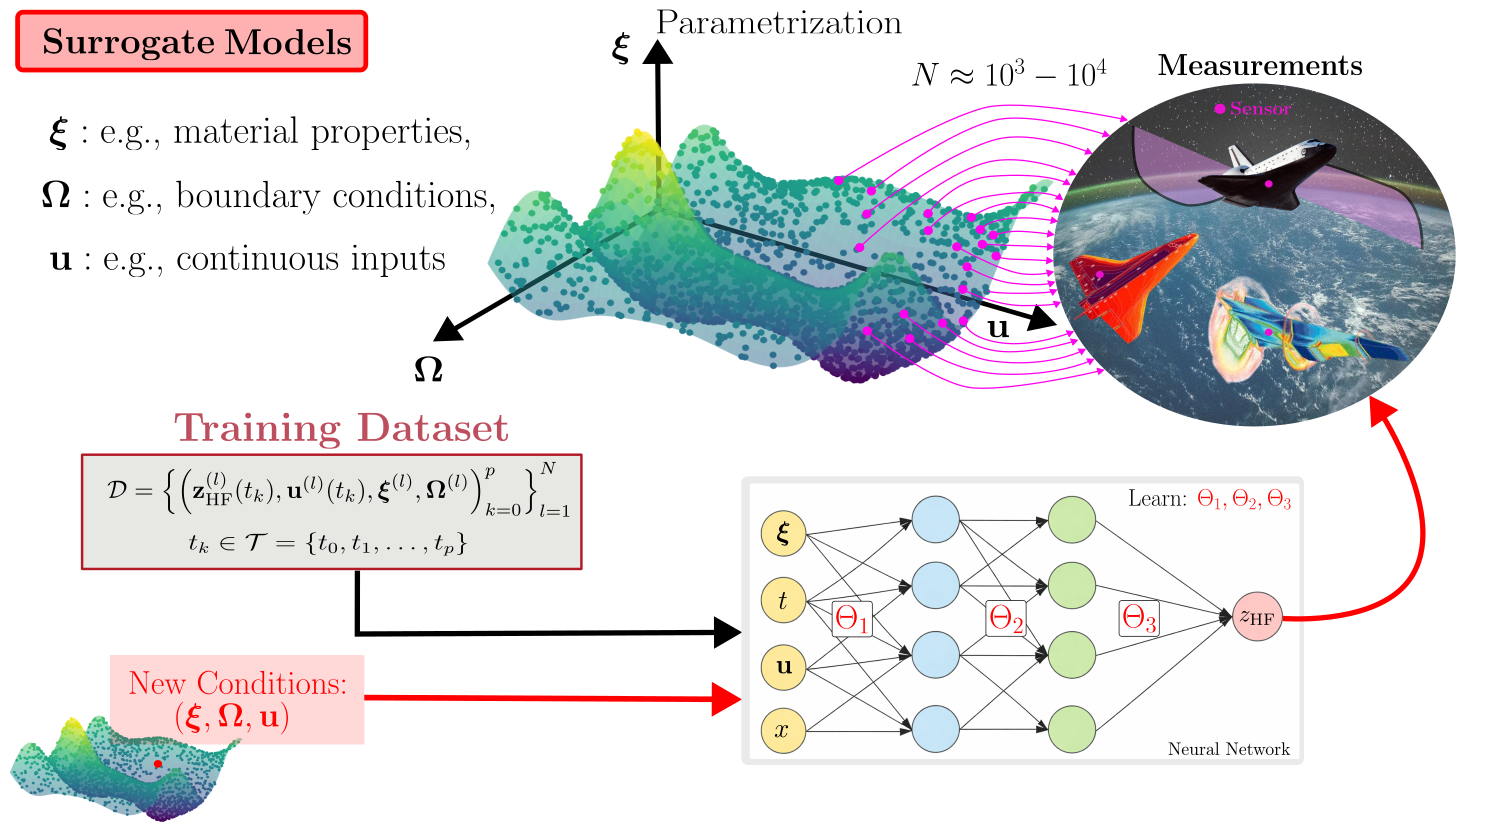
\includegraphics[width=0.9\textwidth]{../figs/sota/surrogates_6.png}
% %     \end{figure}}
% %     \only<7>{
% %     \begin{figure}
% %         \centering
% %         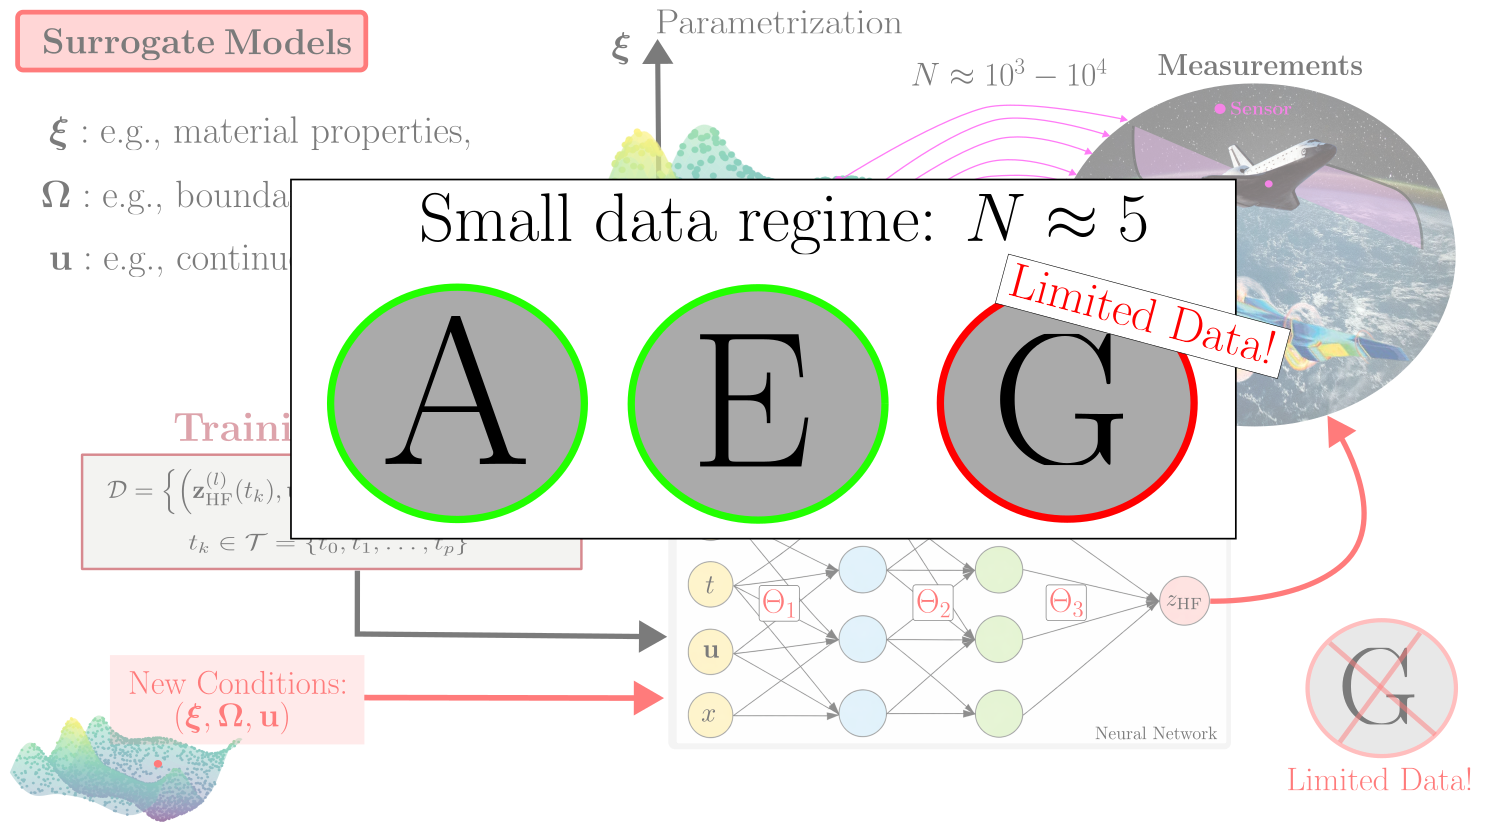
\includegraphics[width=0.9\textwidth]{../figs/sota/surrogates_7.png}
% %     \end{figure}}
% % \end{frame}

% \begin{frame}{\small Persistent issues with \textbf{state-of-the-art} approaches,}
%     \vspace*{-0.2in}
%     \footnotesize
%     \only<1>{
%     \begin{figure}
%         \centering
%         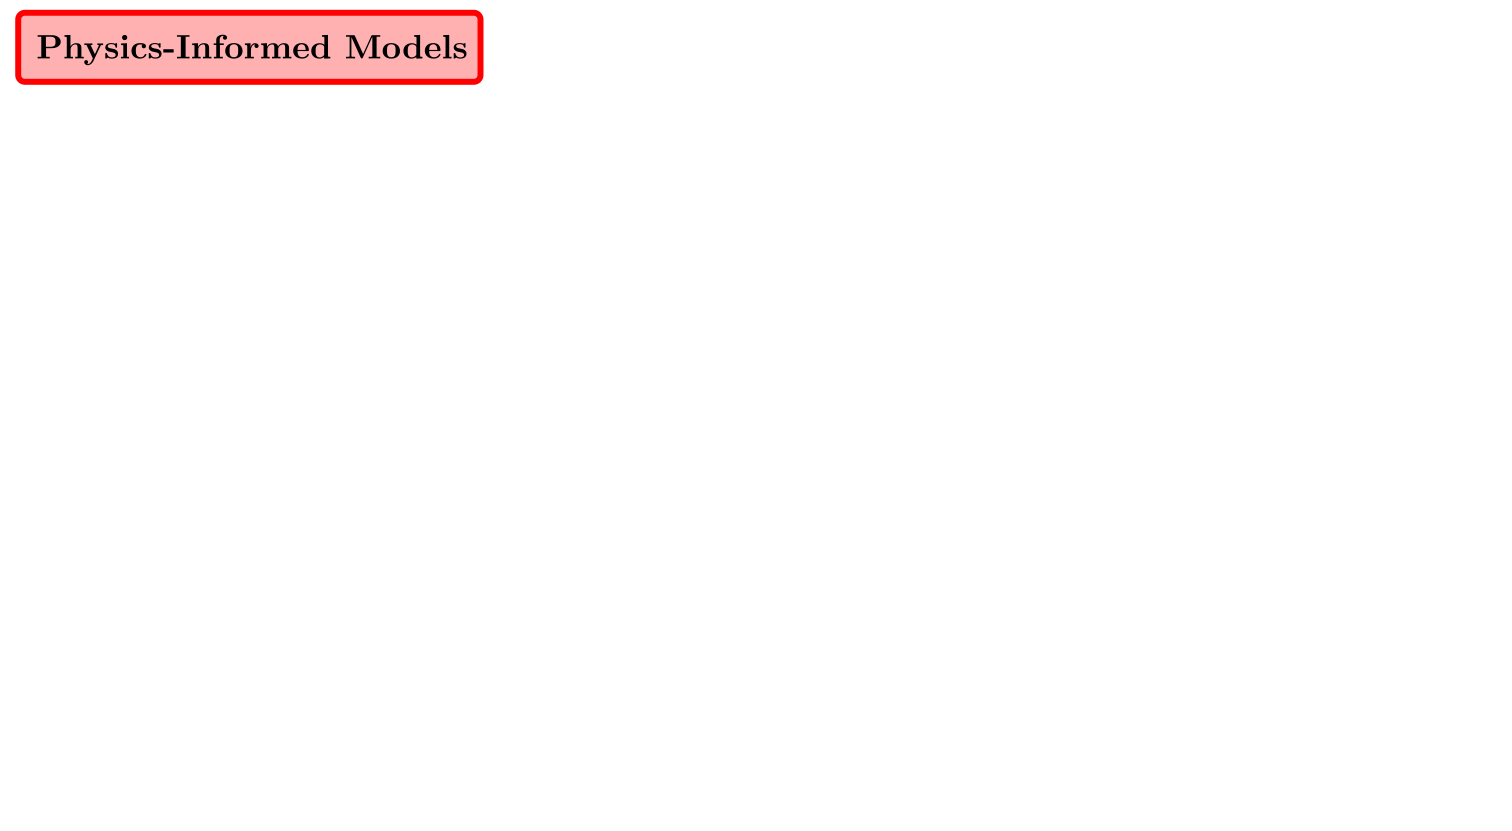
\includegraphics[width=0.9\textwidth]{../figs/sota/physics_informed_1.png}
%     \end{figure}}
%     \only<2>{
%     \begin{figure}
%         \centering
%         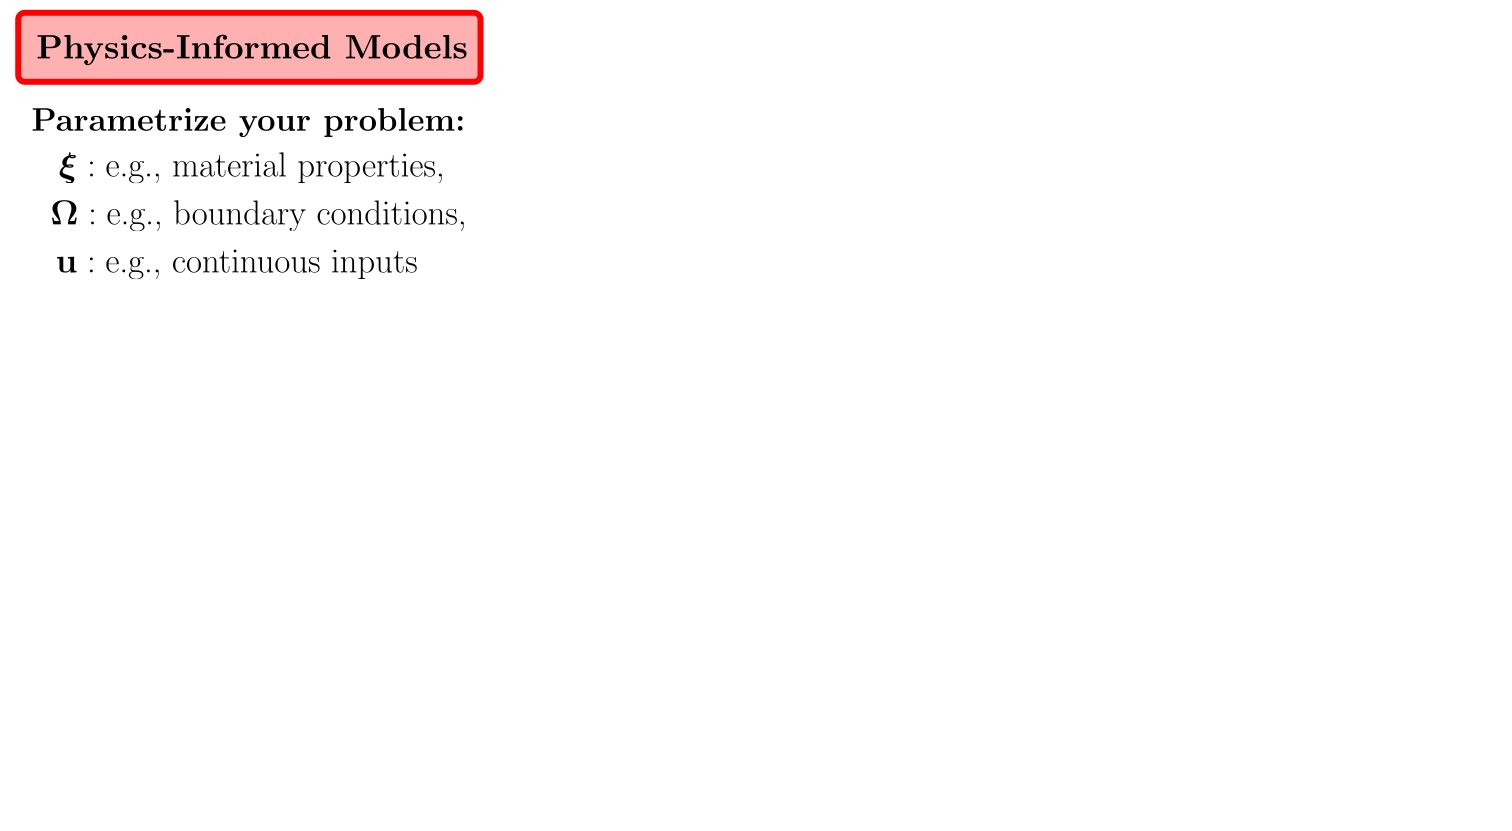
\includegraphics[width=0.9\textwidth]{../figs/sota/physics_informed_2.png}
%     \end{figure}}
%     \only<3>{
%     \begin{figure}
%         \centering
%         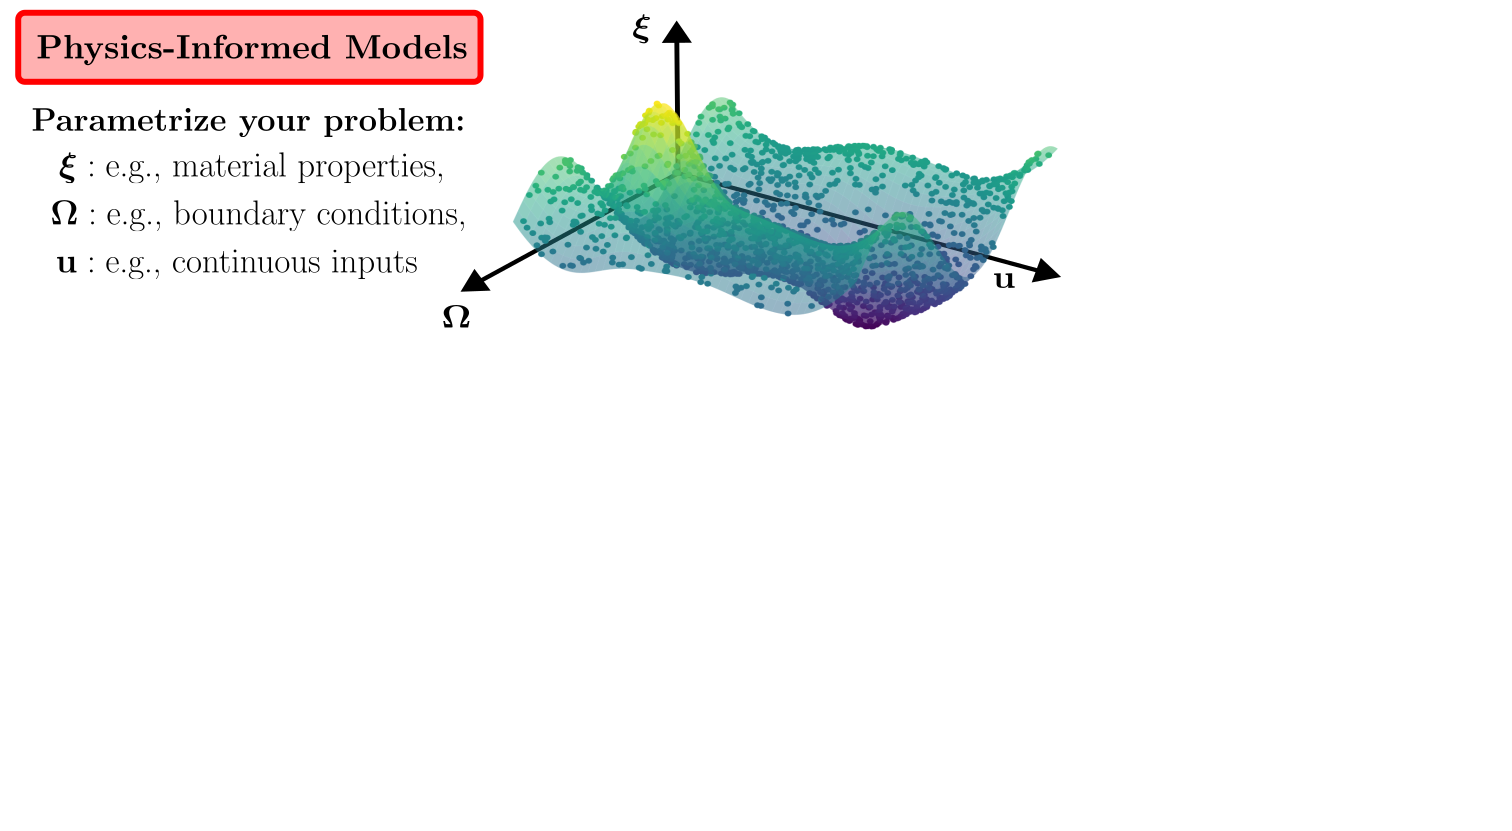
\includegraphics[width=0.9\textwidth]{../figs/sota/physics_informed_3.png}
%     \end{figure}}
%     \only<4>{
%     \begin{figure}
%         \centering
%         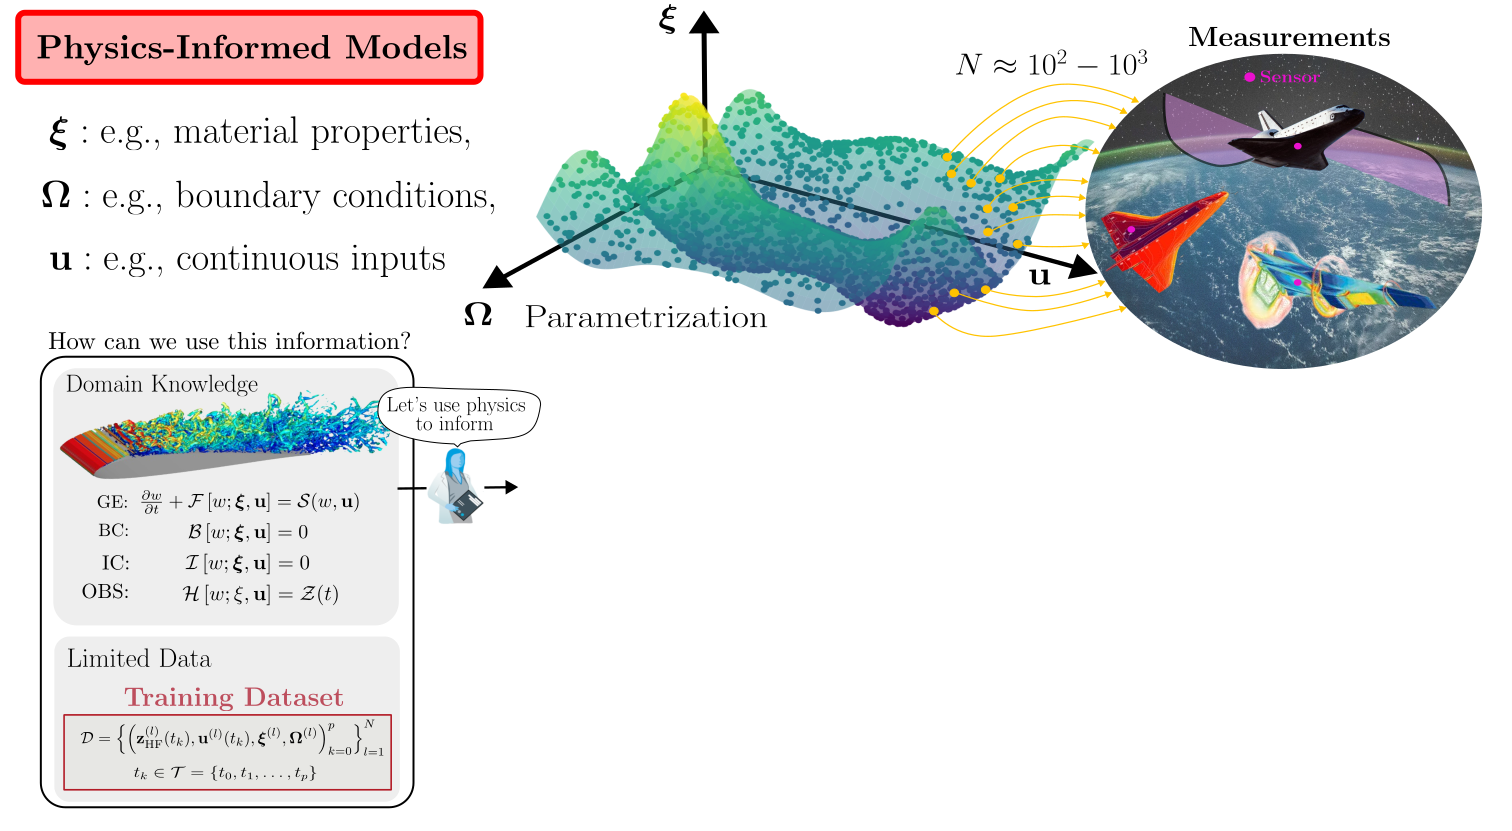
\includegraphics[width=0.9\textwidth]{../figs/sota/physics_informed_4.png}
%     \end{figure}}
%     \only<5>{
%     \begin{figure}
%         \centering
%         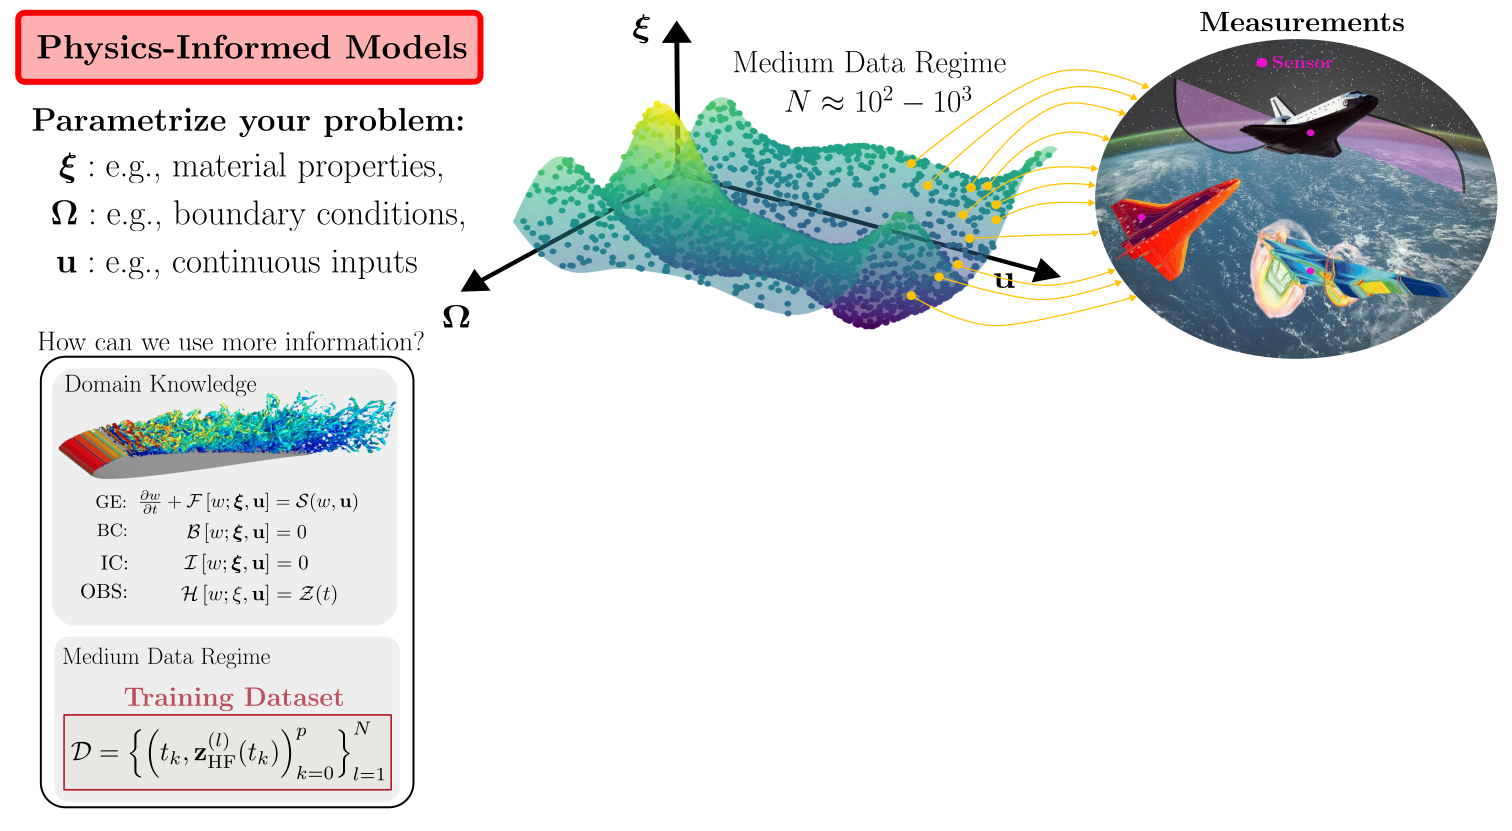
\includegraphics[width=0.9\textwidth]{../figs/sota/physics_informed_5.png}
%     \end{figure}}
%     \only<6>{
%     \begin{figure}
%         \centering
%         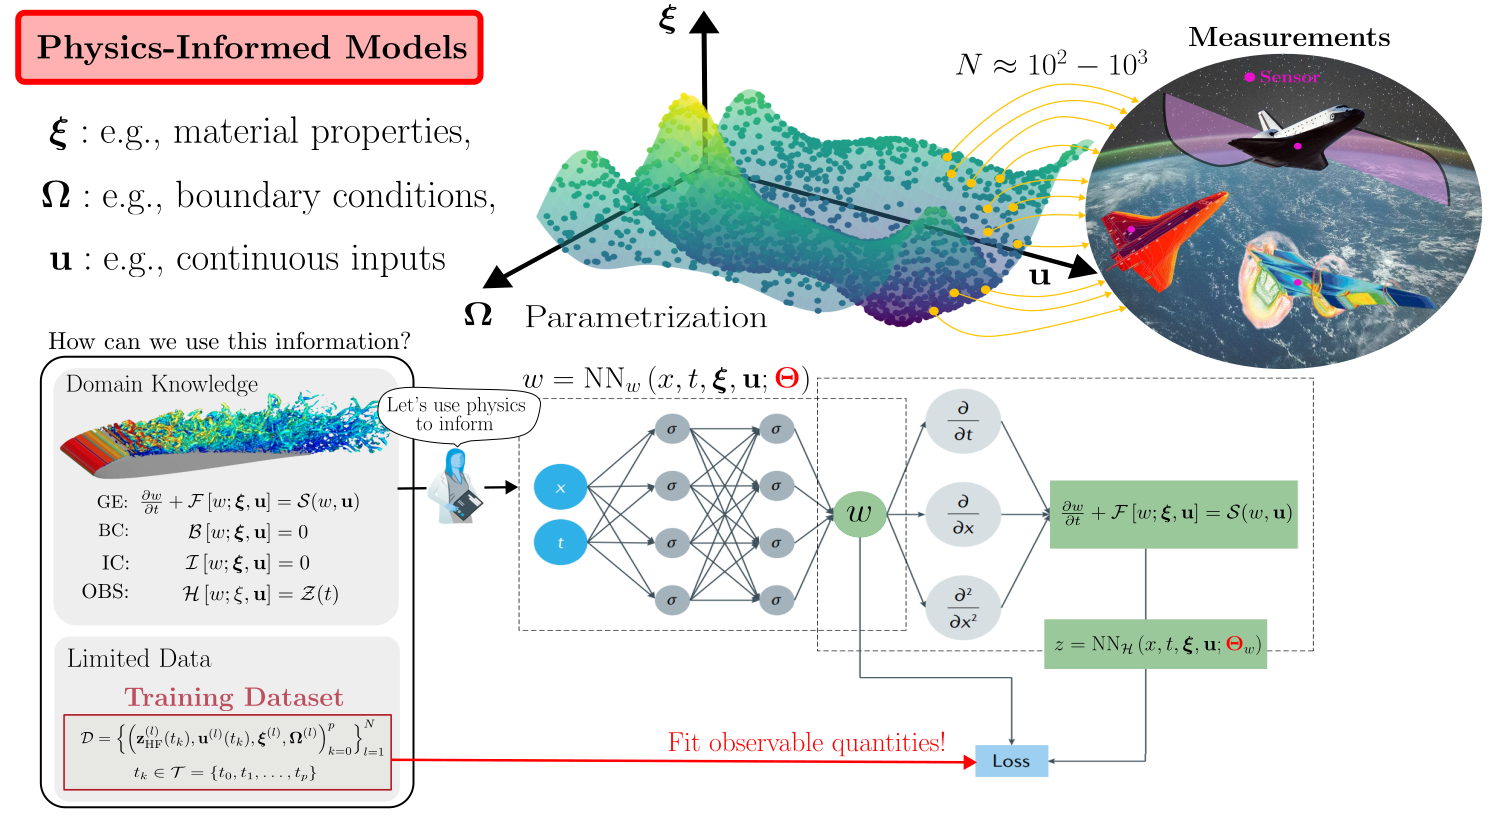
\includegraphics[width=0.9\textwidth]{../figs/sota/physics_informed_6.png}
%     \end{figure}}
%     \only<7>{
%     \begin{figure}
%         \centering
%         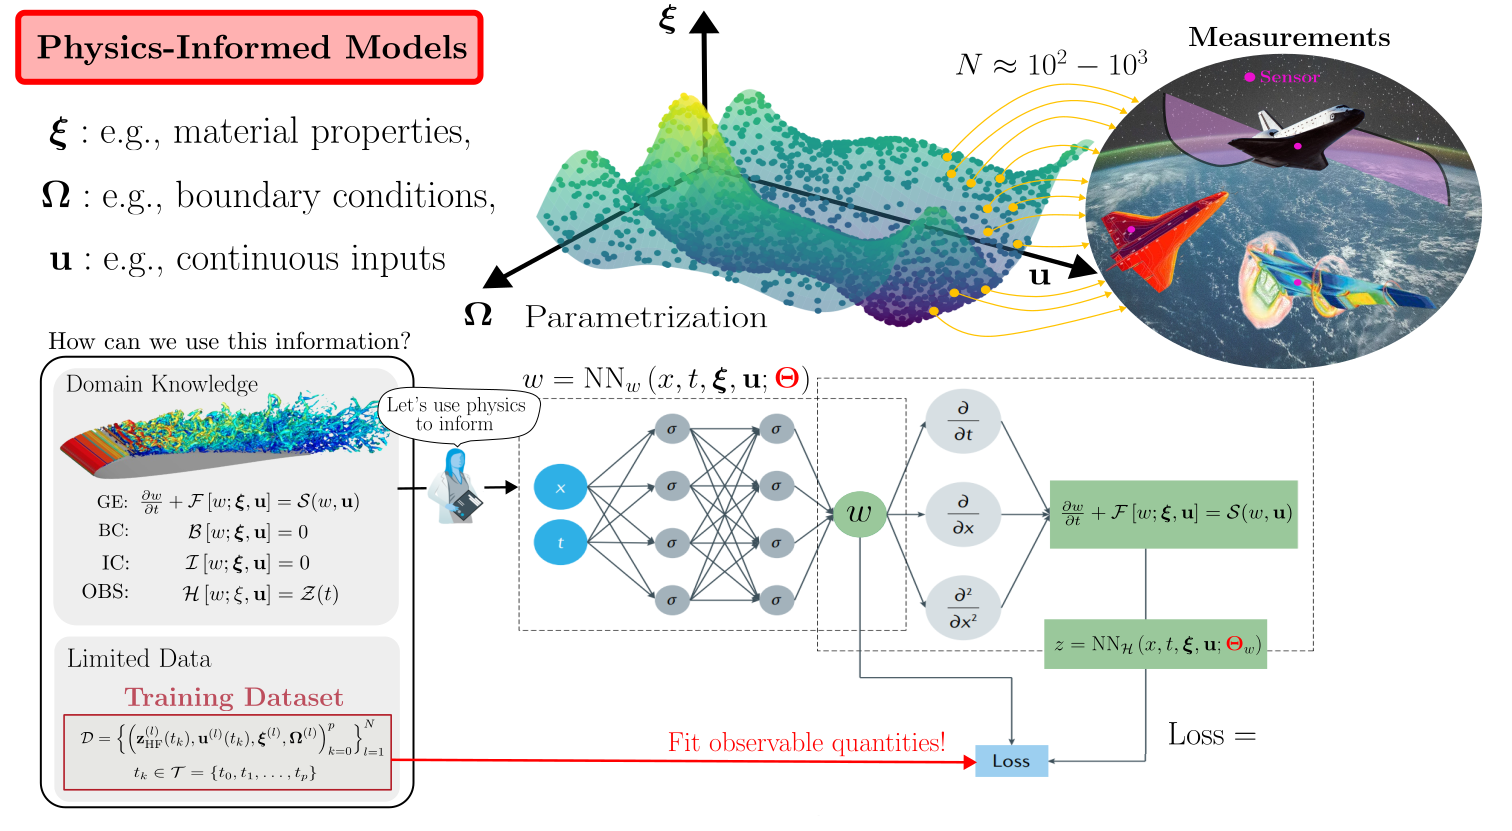
\includegraphics[width=0.9\textwidth]{../figs/sota/physics_informed_7.png}
%     \end{figure}}
%     \only<8>{
%     \begin{figure}
%         \centering
%         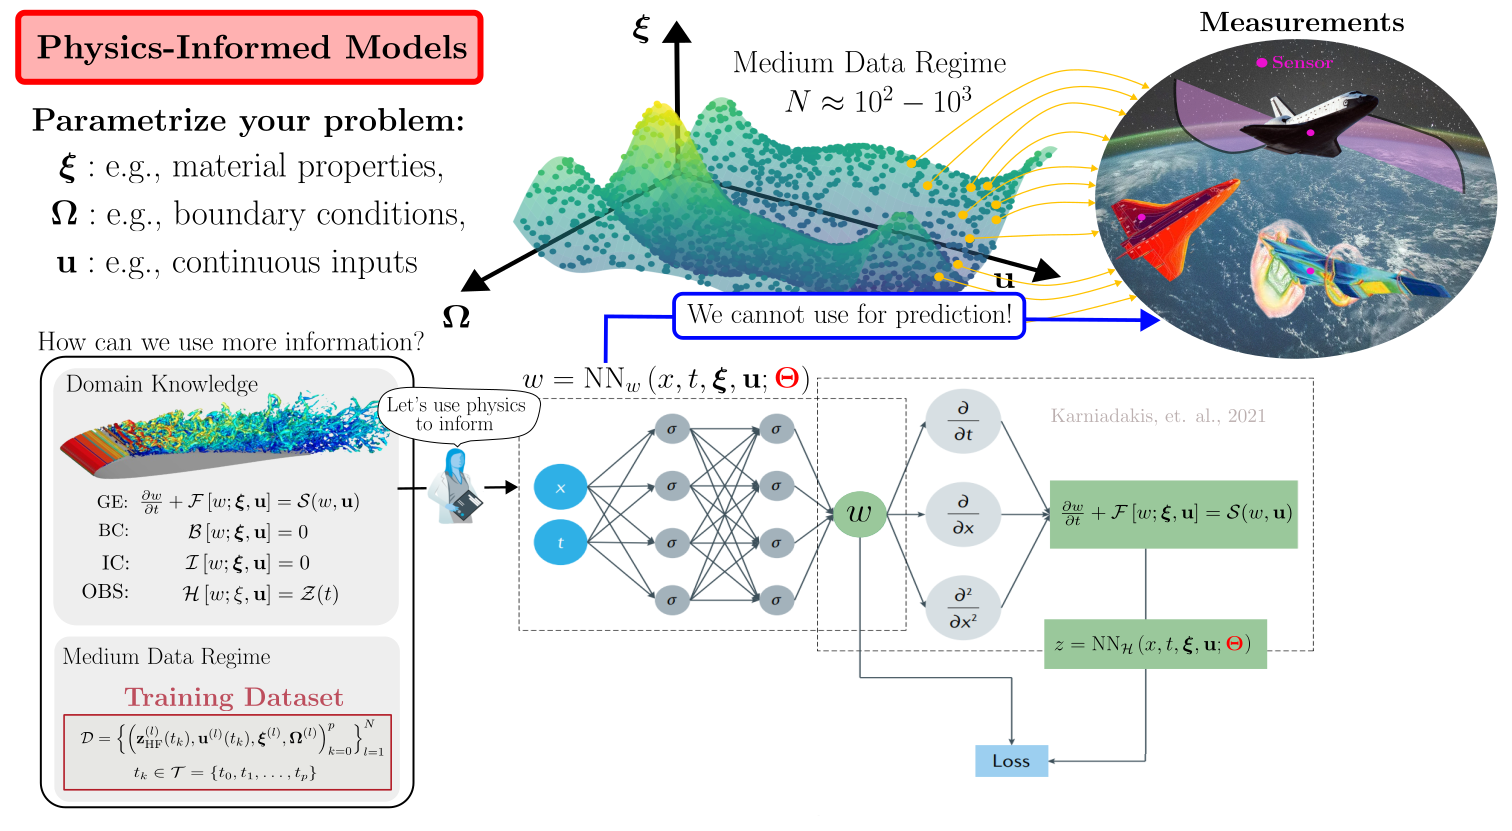
\includegraphics[width=0.9\textwidth]{../figs/sota/physics_informed_8.png}
%     \end{figure}}
%     \only<9>{
%     \begin{figure}
%         \centering
%         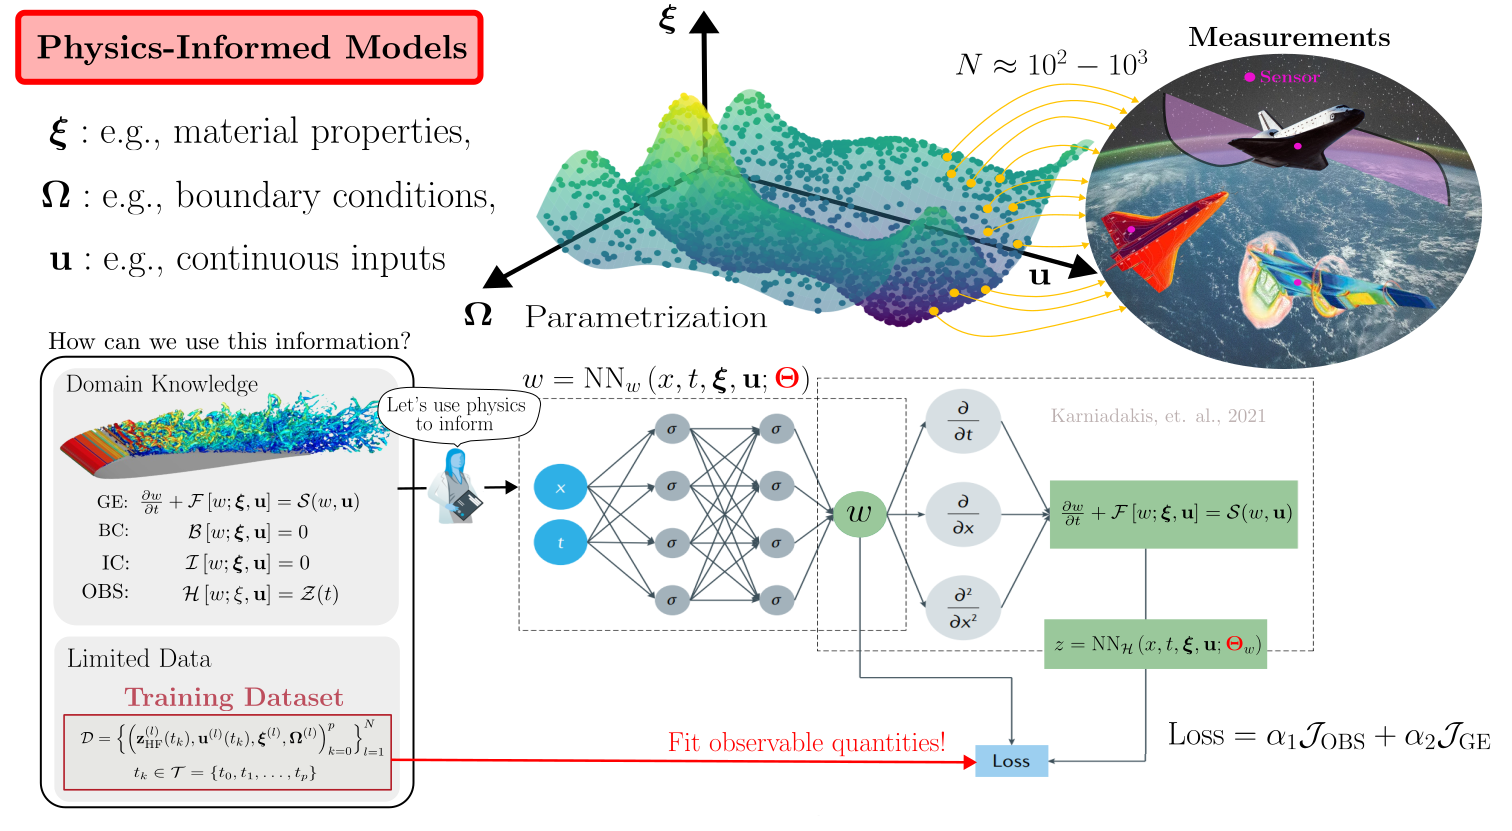
\includegraphics[width=0.9\textwidth]{../figs/sota/physics_informed_9.png}
%     \end{figure}}
%     \only<10>{
%     \begin{figure}
%         \centering
%         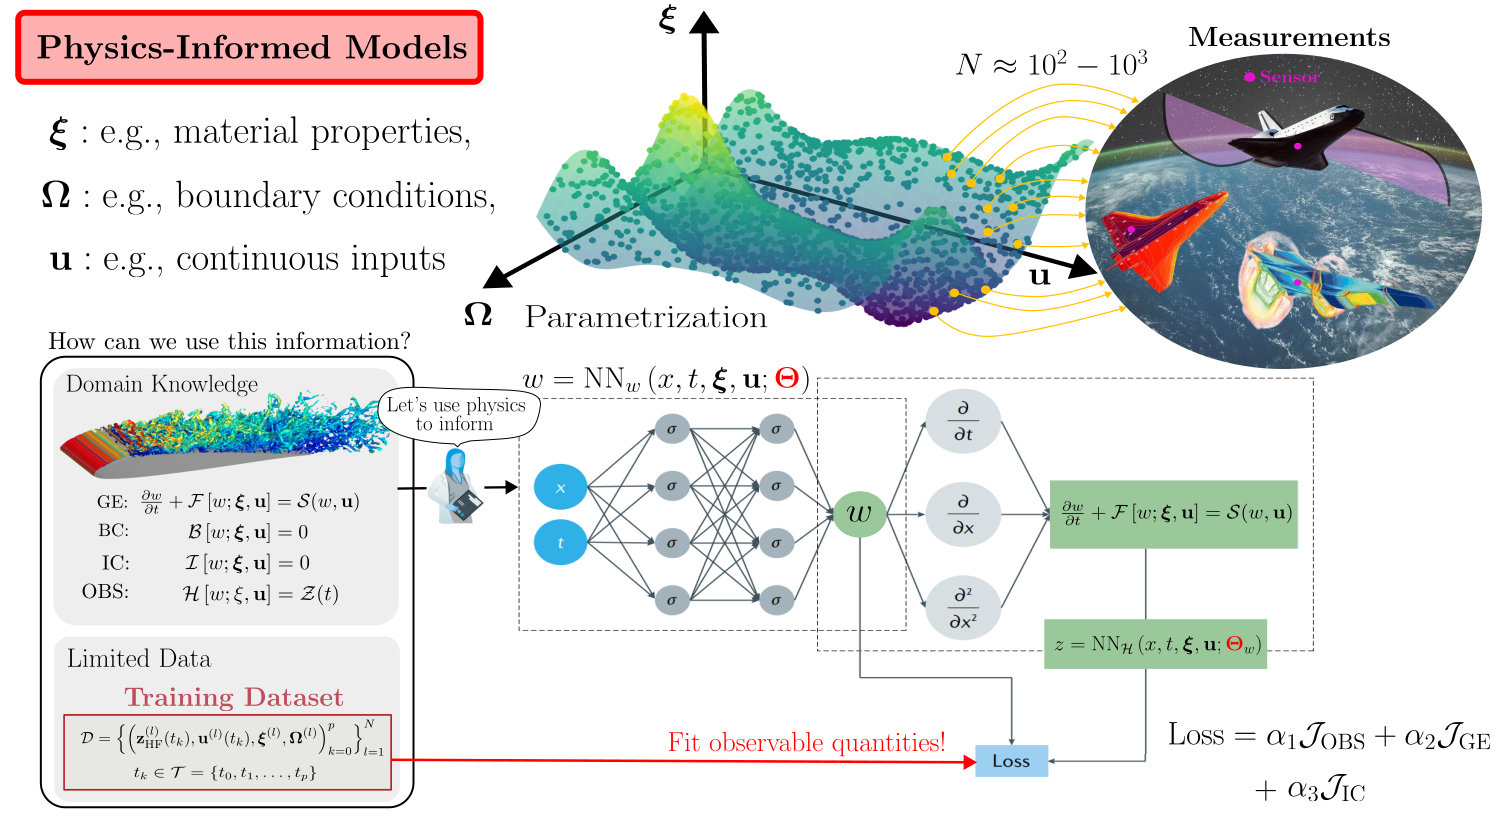
\includegraphics[width=0.9\textwidth]{../figs/sota/physics_informed_10.png}
%     \end{figure}}
%     \only<11>{
%     \begin{figure}
%         \centering
%         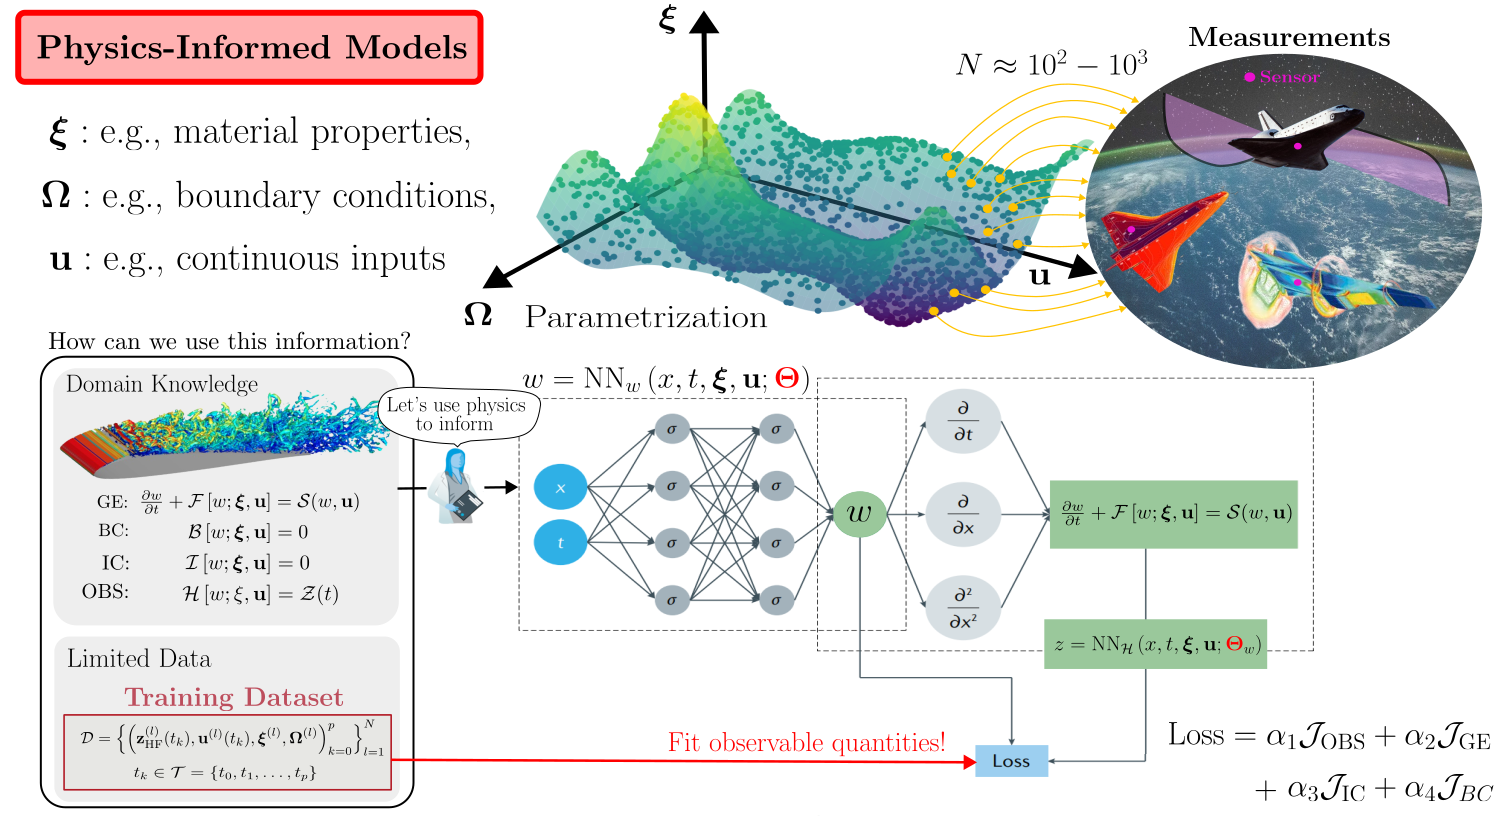
\includegraphics[width=0.9\textwidth]{../figs/sota/physics_informed_11.png}
%     \end{figure}}
%     \only<12>{
%     \begin{figure}
%         \centering
%         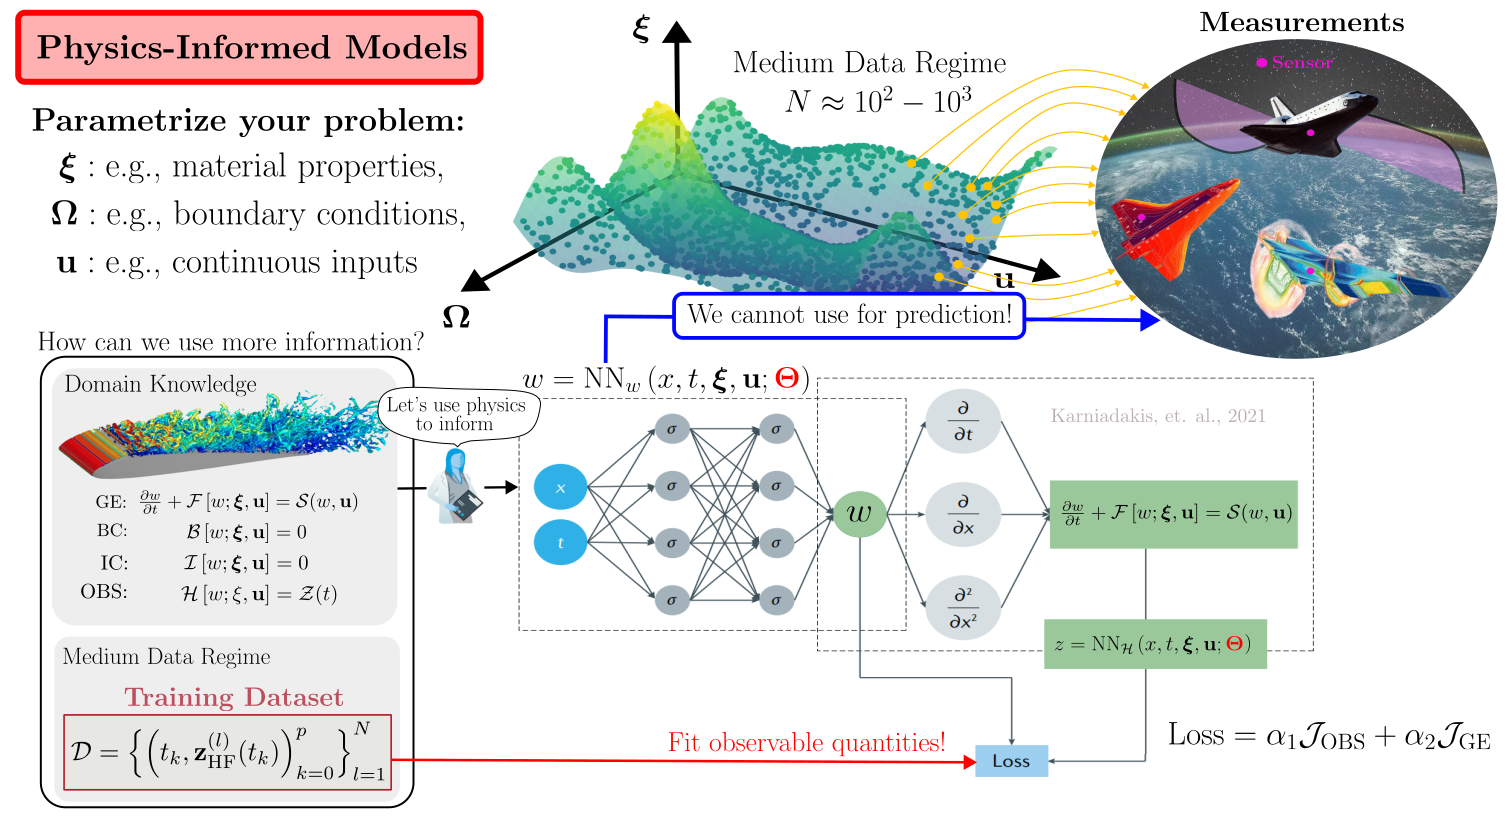
\includegraphics[width=0.9\textwidth]{../figs/sota/physics_informed_12.png}
%     \end{figure}}
%     \only<13>{
%     \begin{figure}
%         \centering
%         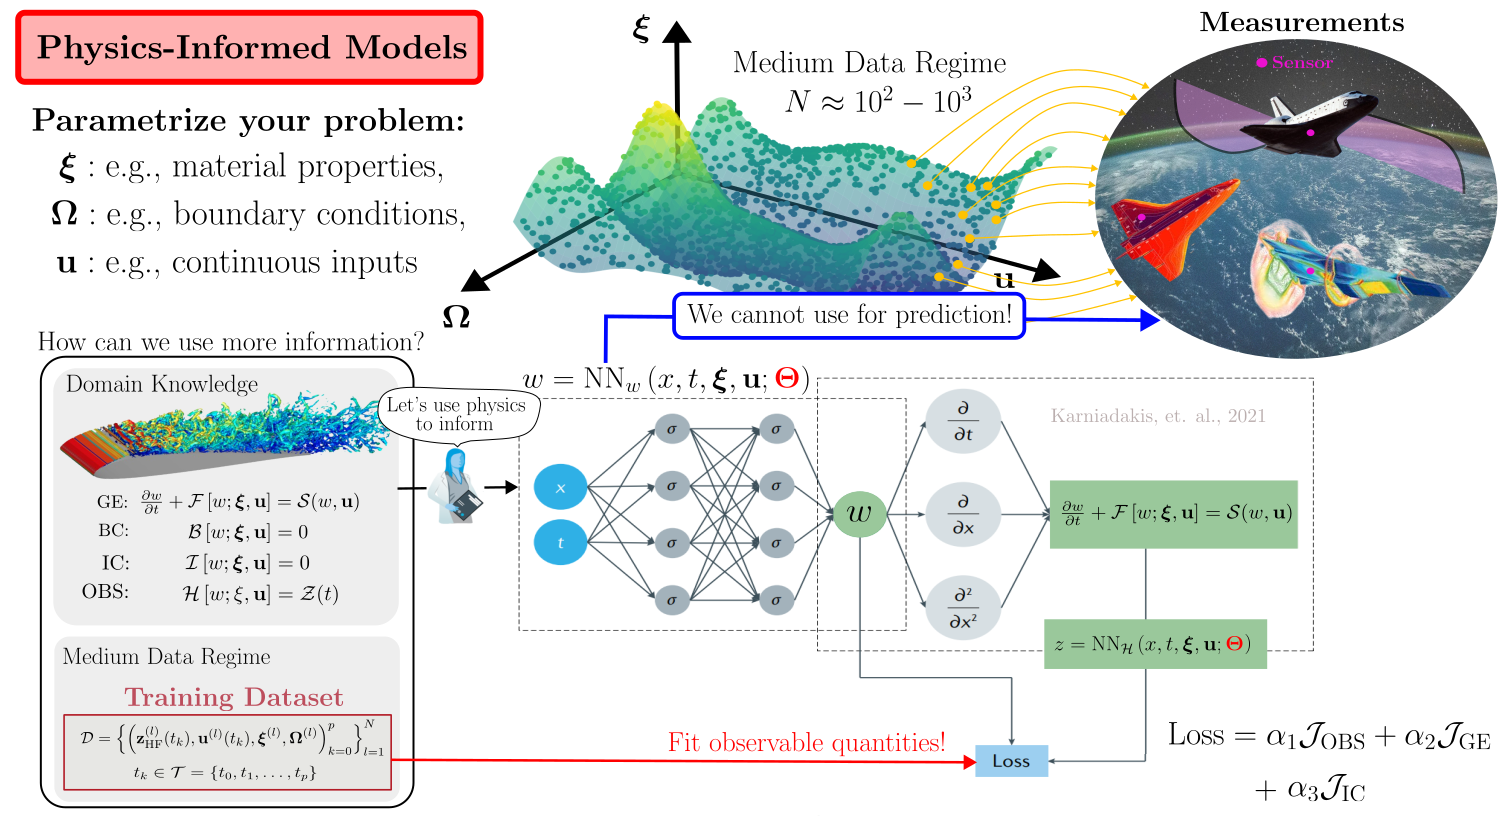
\includegraphics[width=0.9\textwidth]{../figs/sota/physics_informed_13.png}
%     \end{figure}}
%     \only<14>{
%     \begin{figure}
%         \centering
%         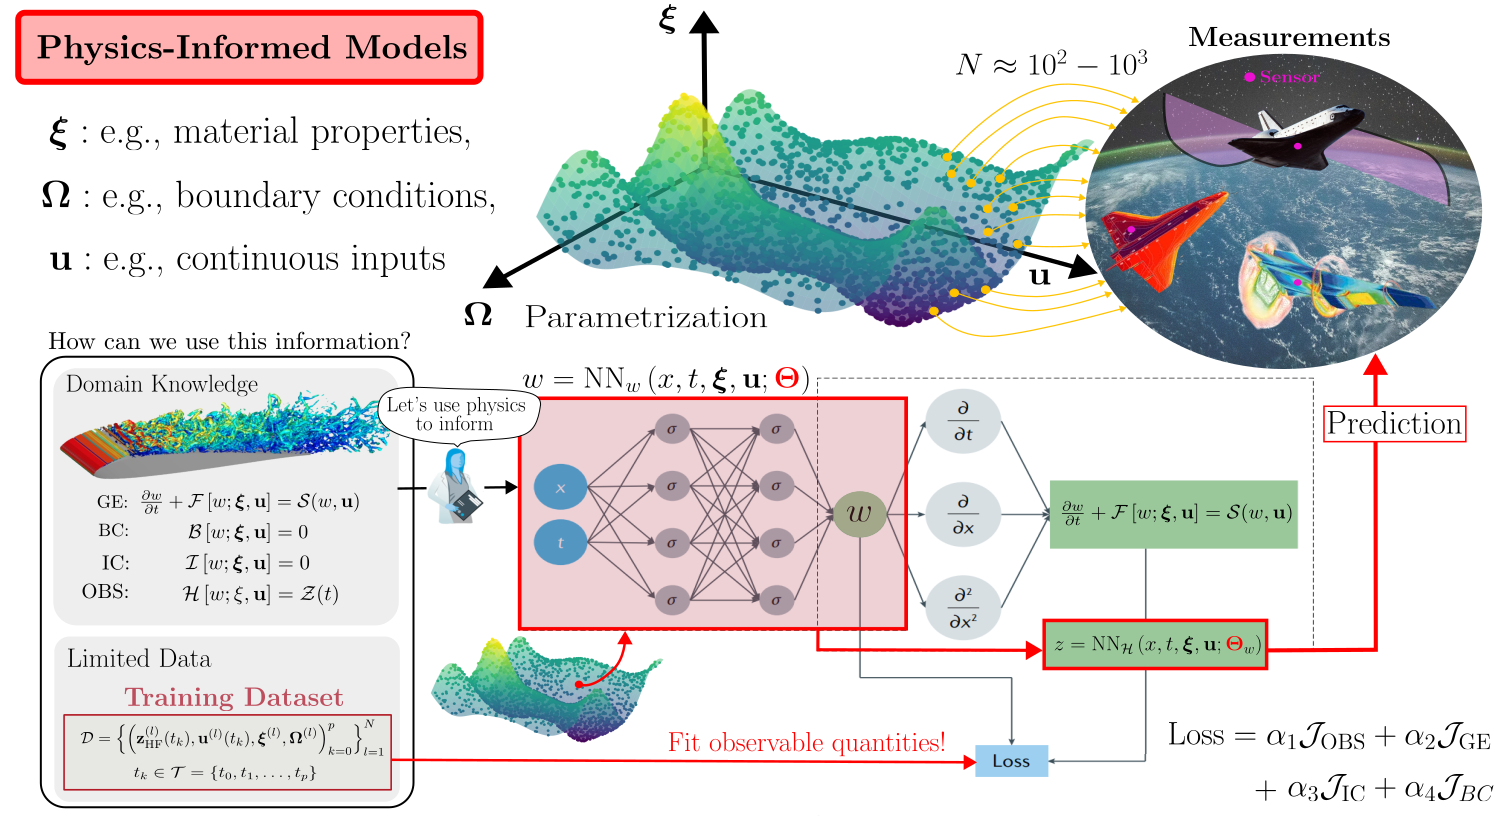
\includegraphics[width=0.9\textwidth]{../figs/sota/physics_informed_14.png}
%     \end{figure}}
%     \only<15>{
%     \begin{figure}
%         \centering
%         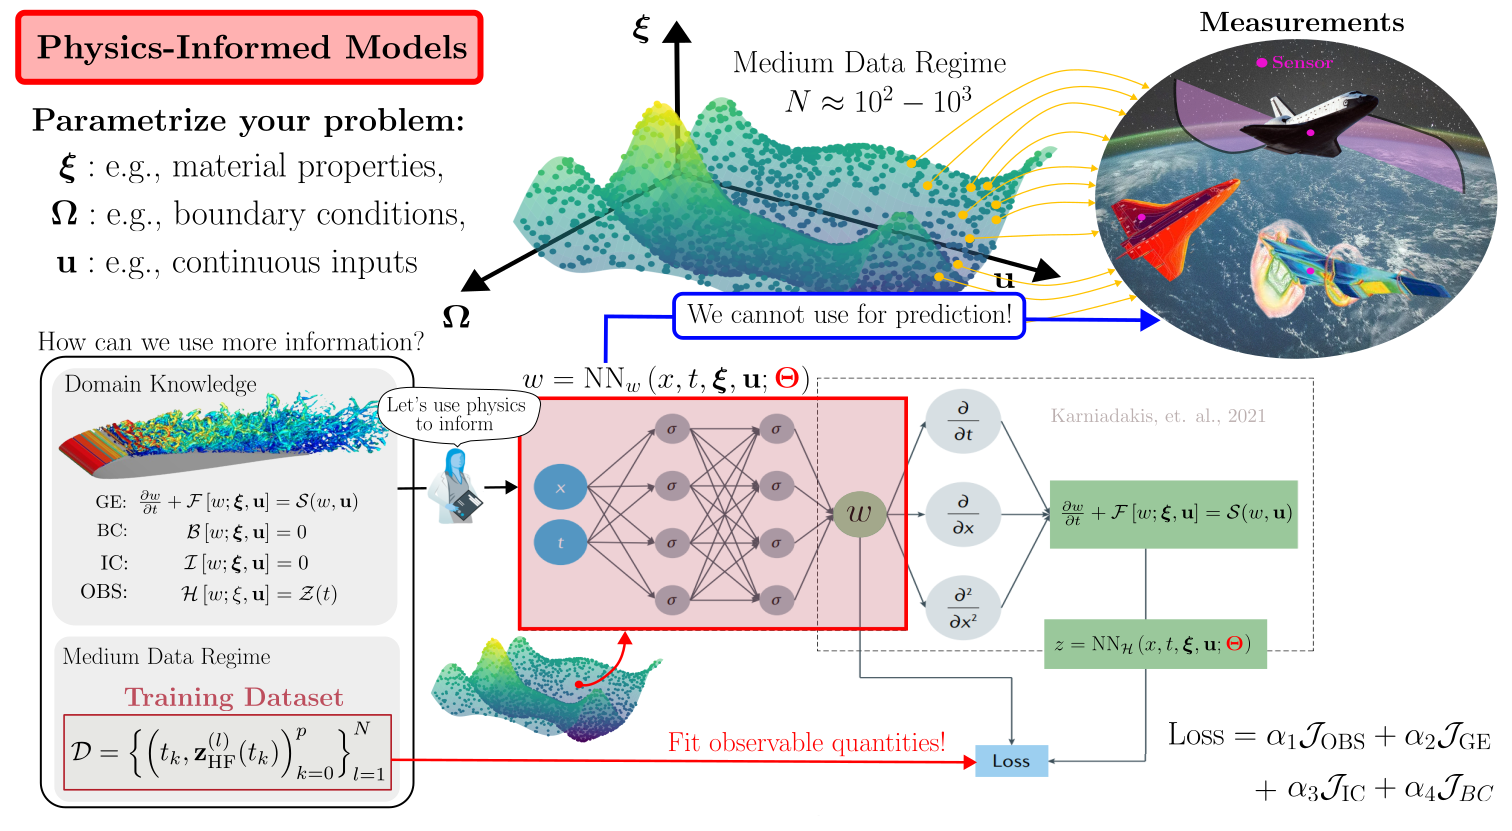
\includegraphics[width=0.9\textwidth]{../figs/sota/physics_informed_15.png}
%     \end{figure}}
%     \begin{center}
%         {\tiny GE: governing equations, BC: boundary conditions, IC: initial conditions, OBS: observable, NN: neural network}
%     \end{center}
% \end{frame}

\begin{frame}{\small So, how does PIROM \textbf{solve the ITM} in \textbf{small-data regimes}?}
    \vspace*{-0.2in}
    \footnotesize
    \only<1>{
    \begin{figure}
        \centering
        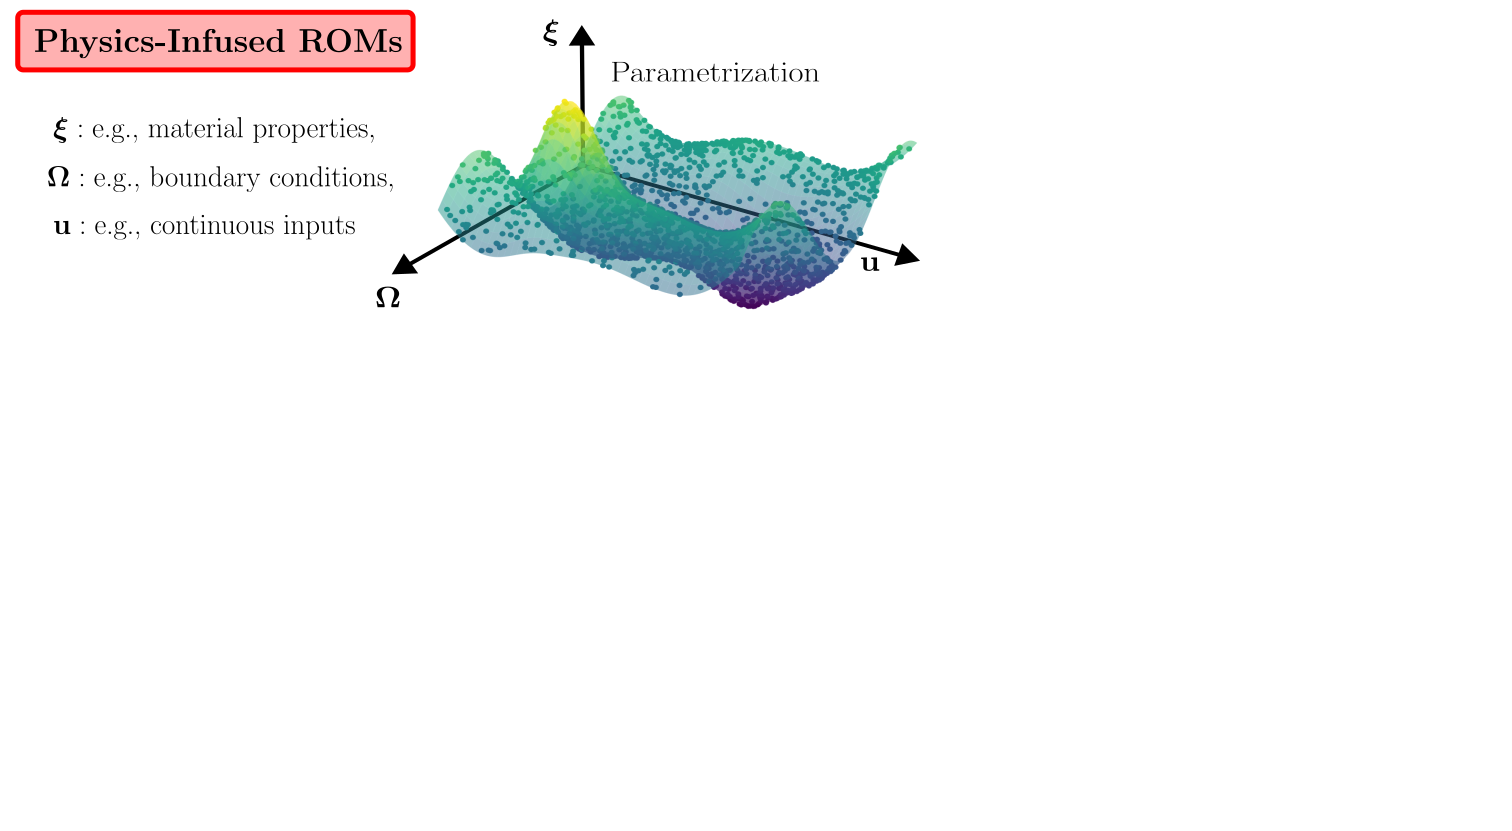
\includegraphics[width=0.9\textwidth]{../figs/sota/physics_infused_1.png}
    \end{figure}}
    \only<2>{
    \begin{figure}
        \centering
        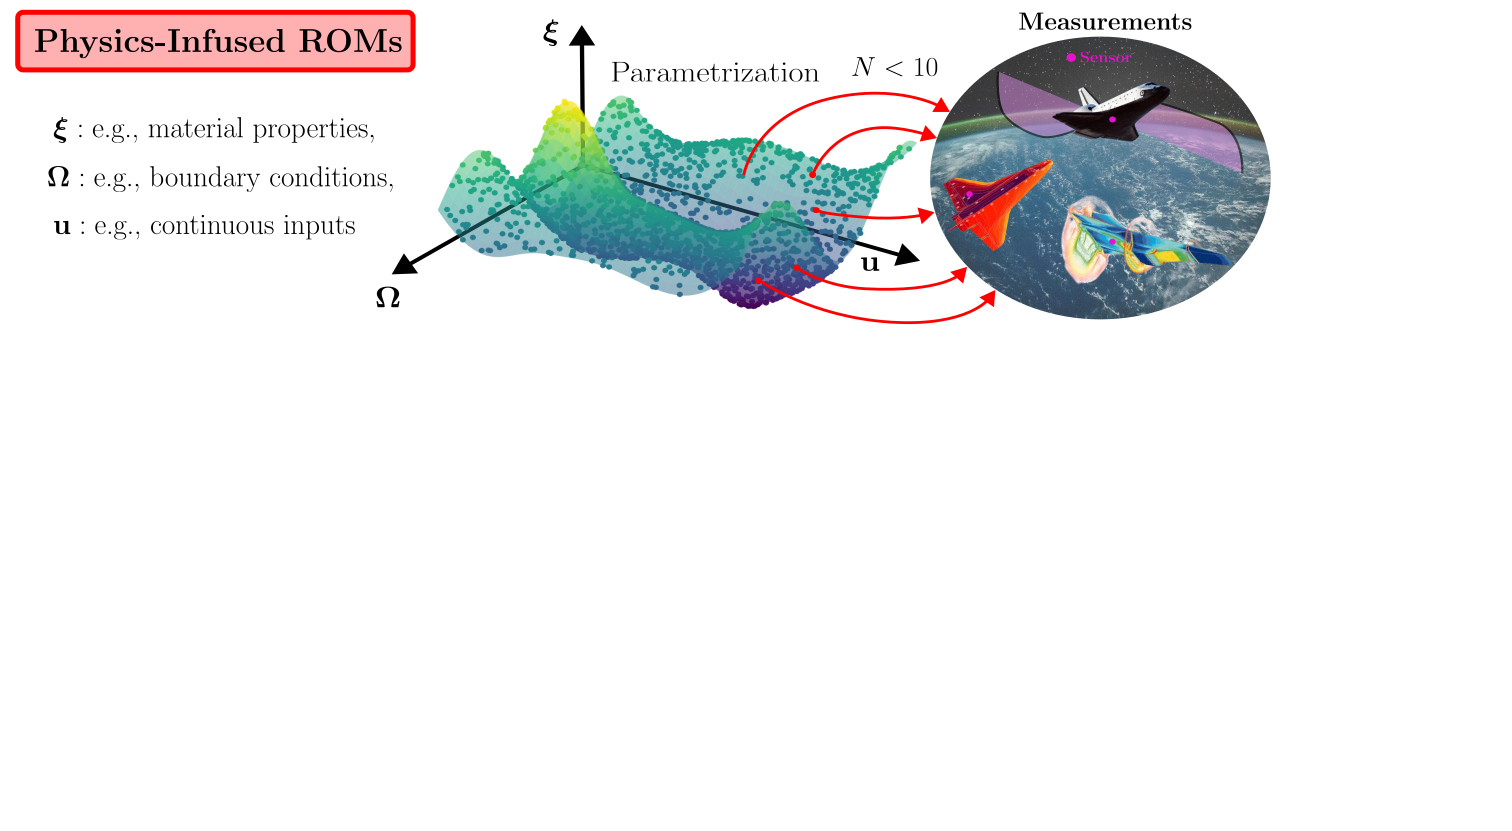
\includegraphics[width=0.9\textwidth]{../figs/sota/physics_infused_2.png}
    \end{figure}}
    \only<3>{
    \begin{figure}
        \centering
        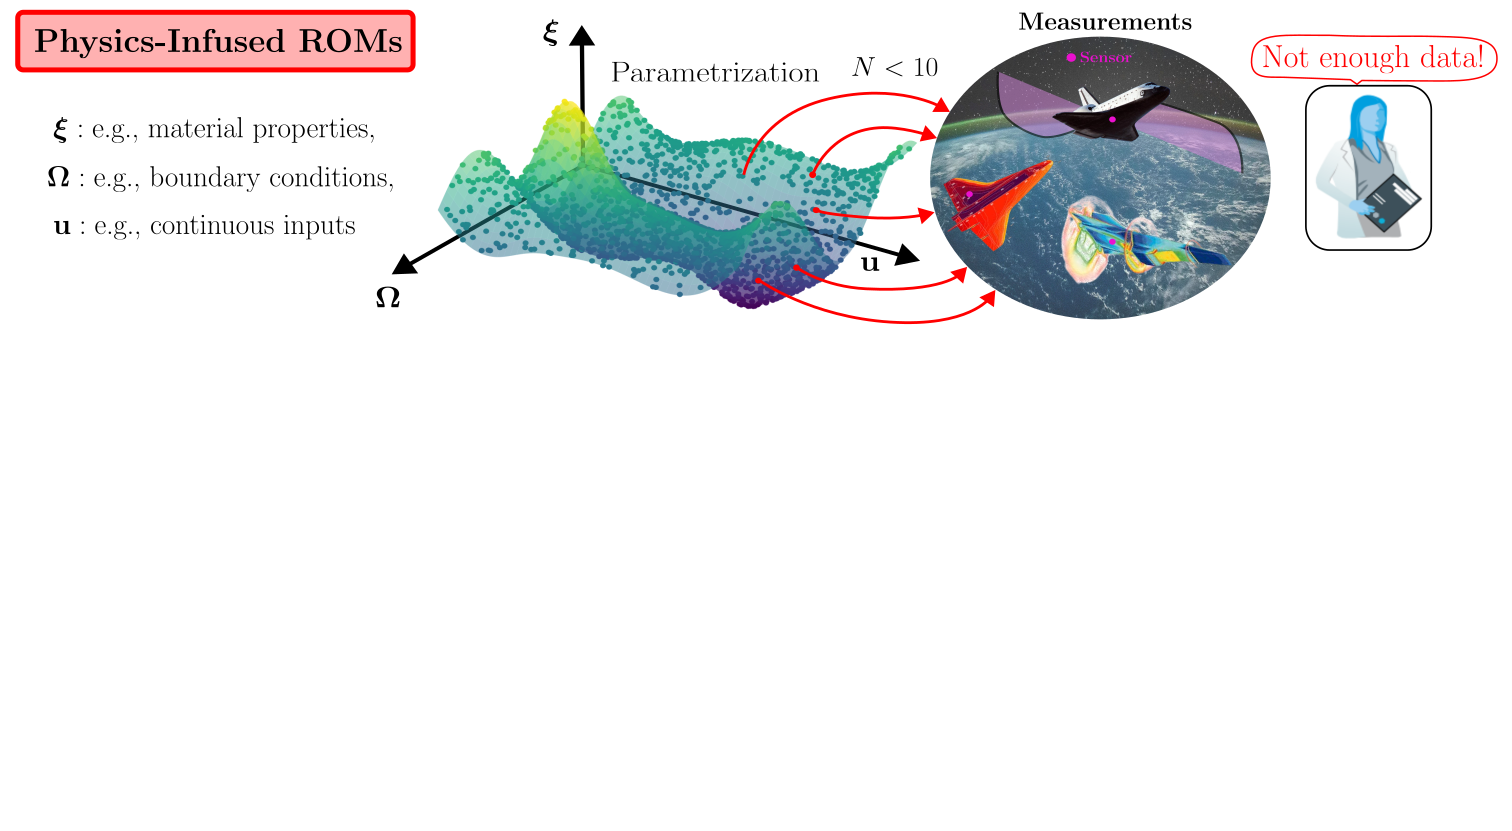
\includegraphics[width=0.9\textwidth]{../figs/sota/physics_infused_3.png}
    \end{figure}}
    \only<4>{
    \begin{figure}
        \centering
        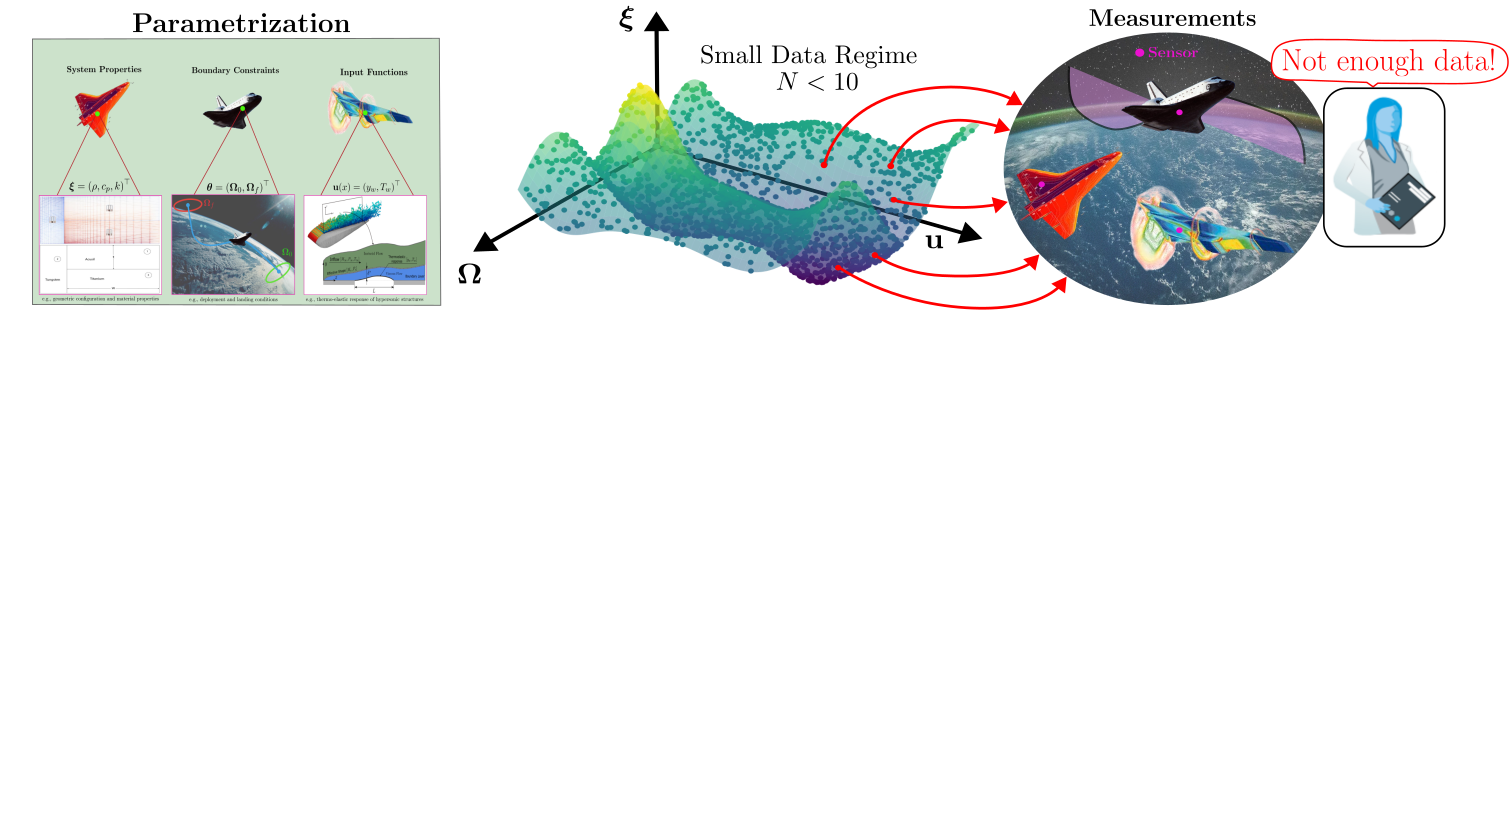
\includegraphics[width=0.9\textwidth]{../figs/sota/physics_infused_4.png}
    \end{figure}}
    \only<5>{
    \begin{figure}
        \centering
        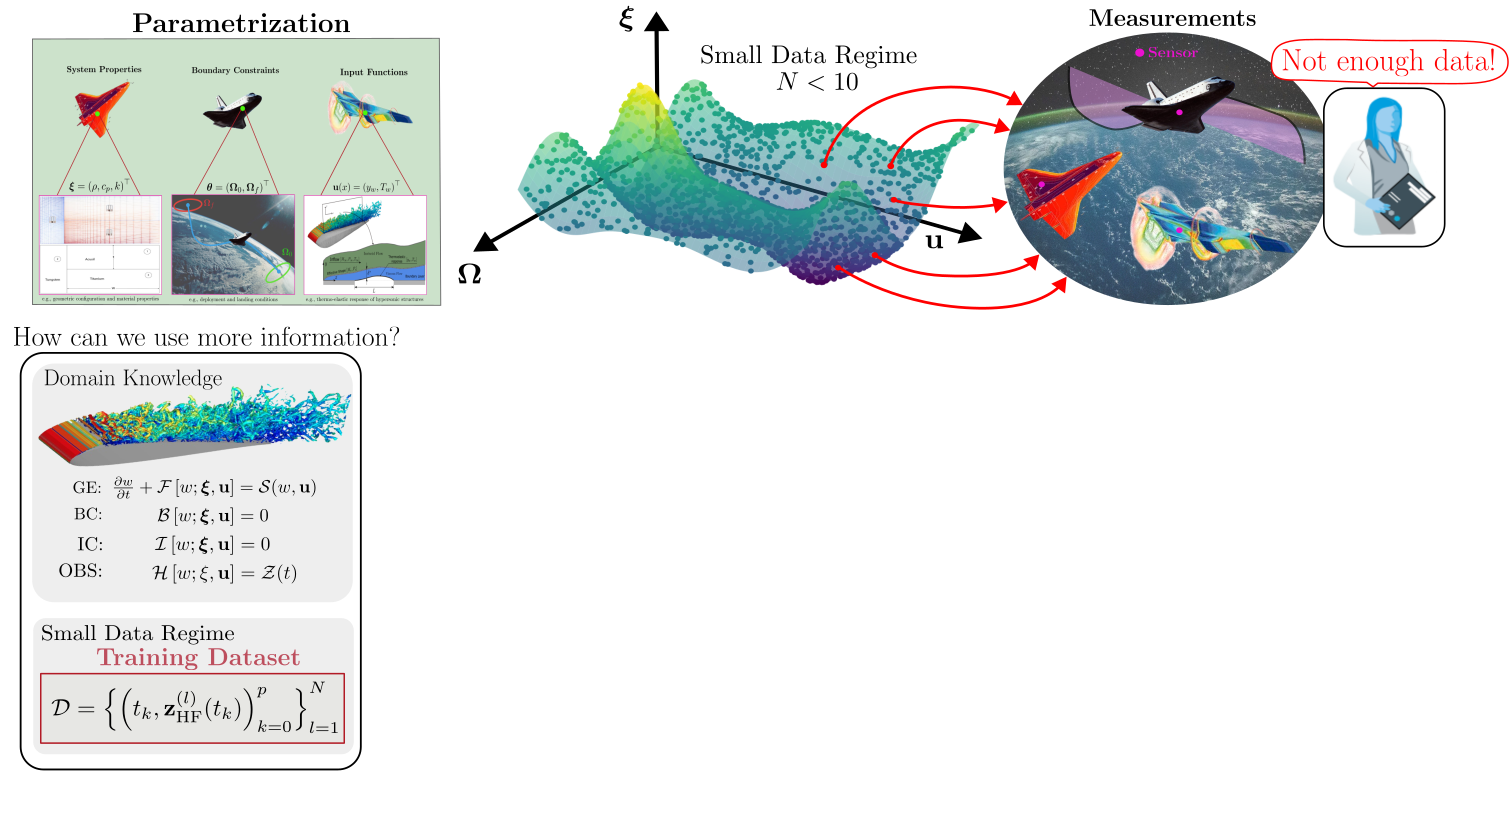
\includegraphics[width=0.9\textwidth]{../figs/sota/physics_infused_5.png}
    \end{figure}}
    \only<6>{
    \begin{figure}
        \centering
        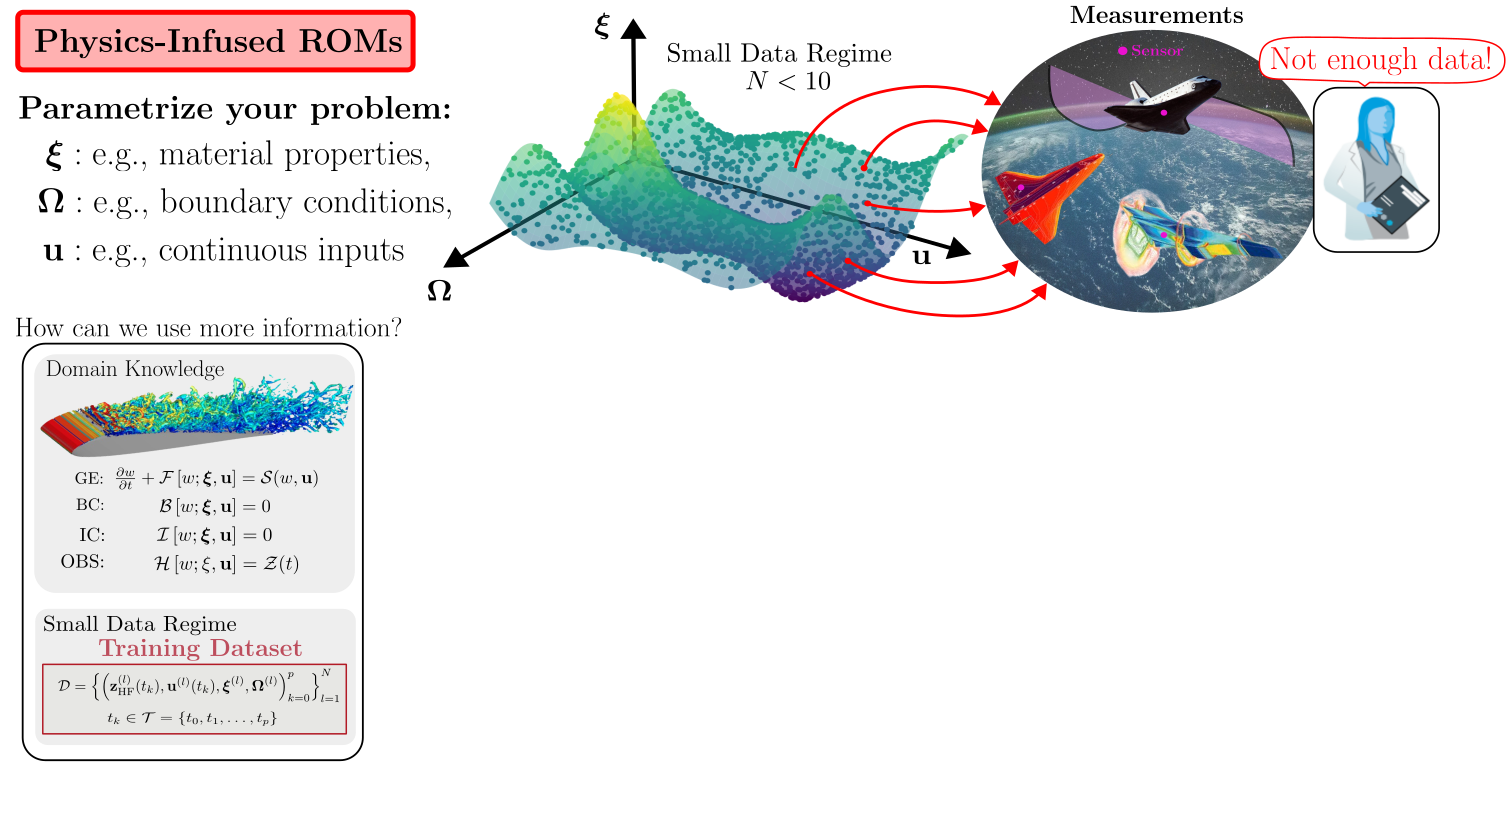
\includegraphics[width=0.9\textwidth]{../figs/sota/physics_infused_6.png}
    \end{figure}}
    \only<7>{
    \begin{figure}
        \centering
        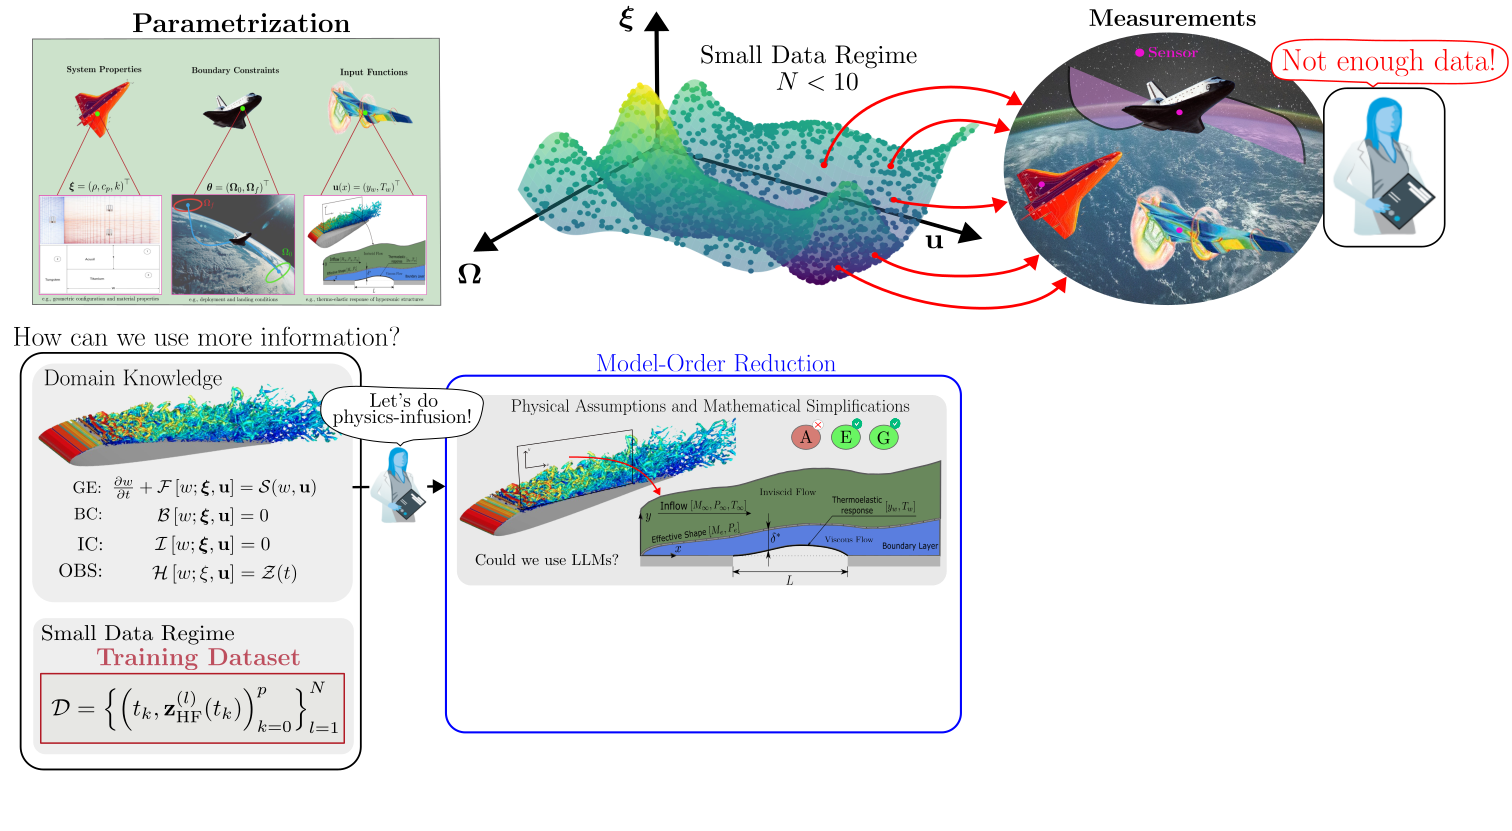
\includegraphics[width=0.9\textwidth]{../figs/sota/physics_infused_7.png}
    \end{figure}}
    \only<8>{
    \begin{figure}
        \centering
        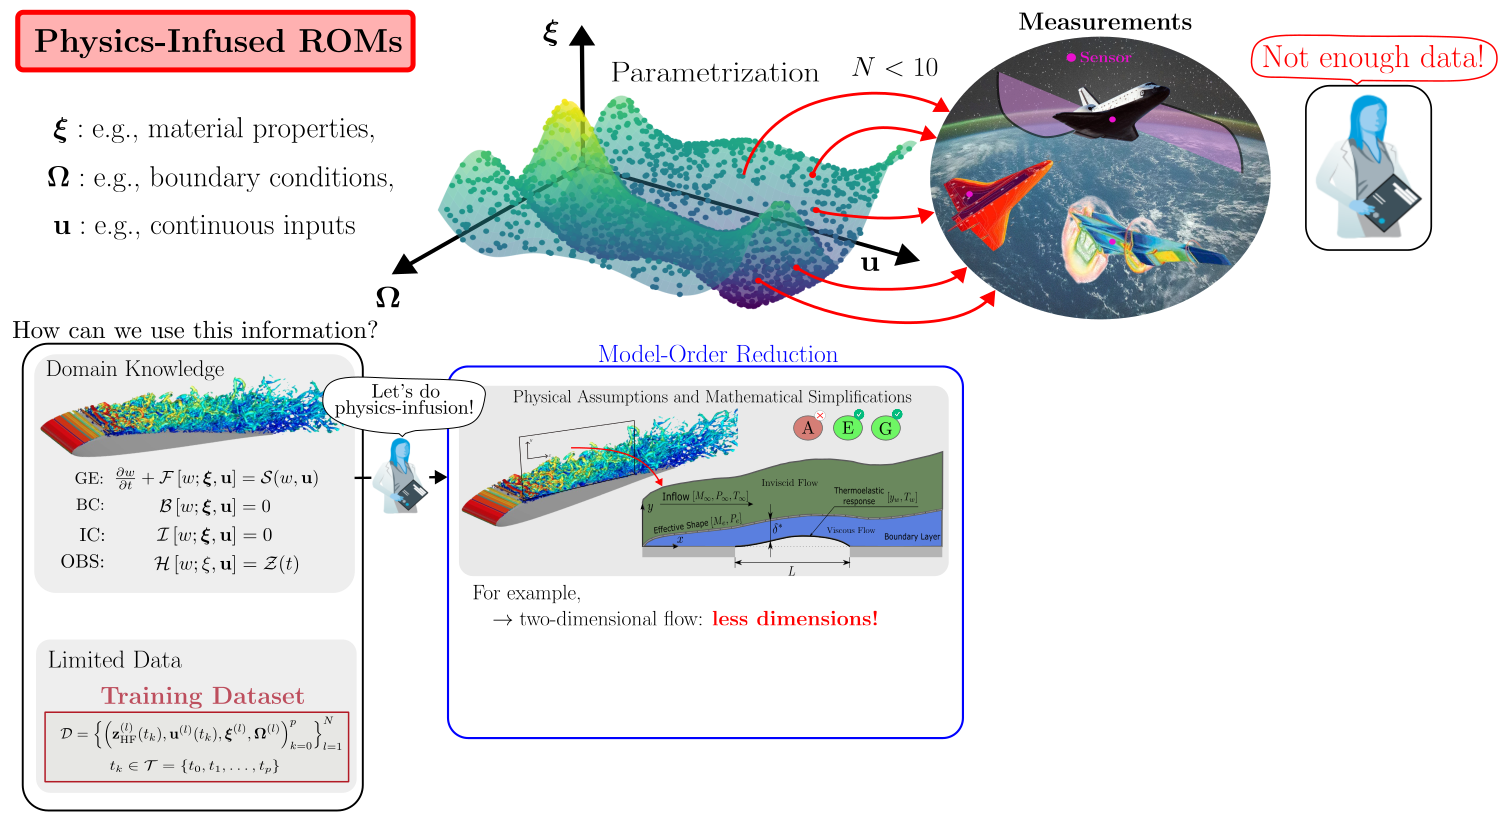
\includegraphics[width=0.9\textwidth]{../figs/sota/physics_infused_8.png}
    \end{figure}}
    \only<9>{
    \begin{figure}
        \centering
        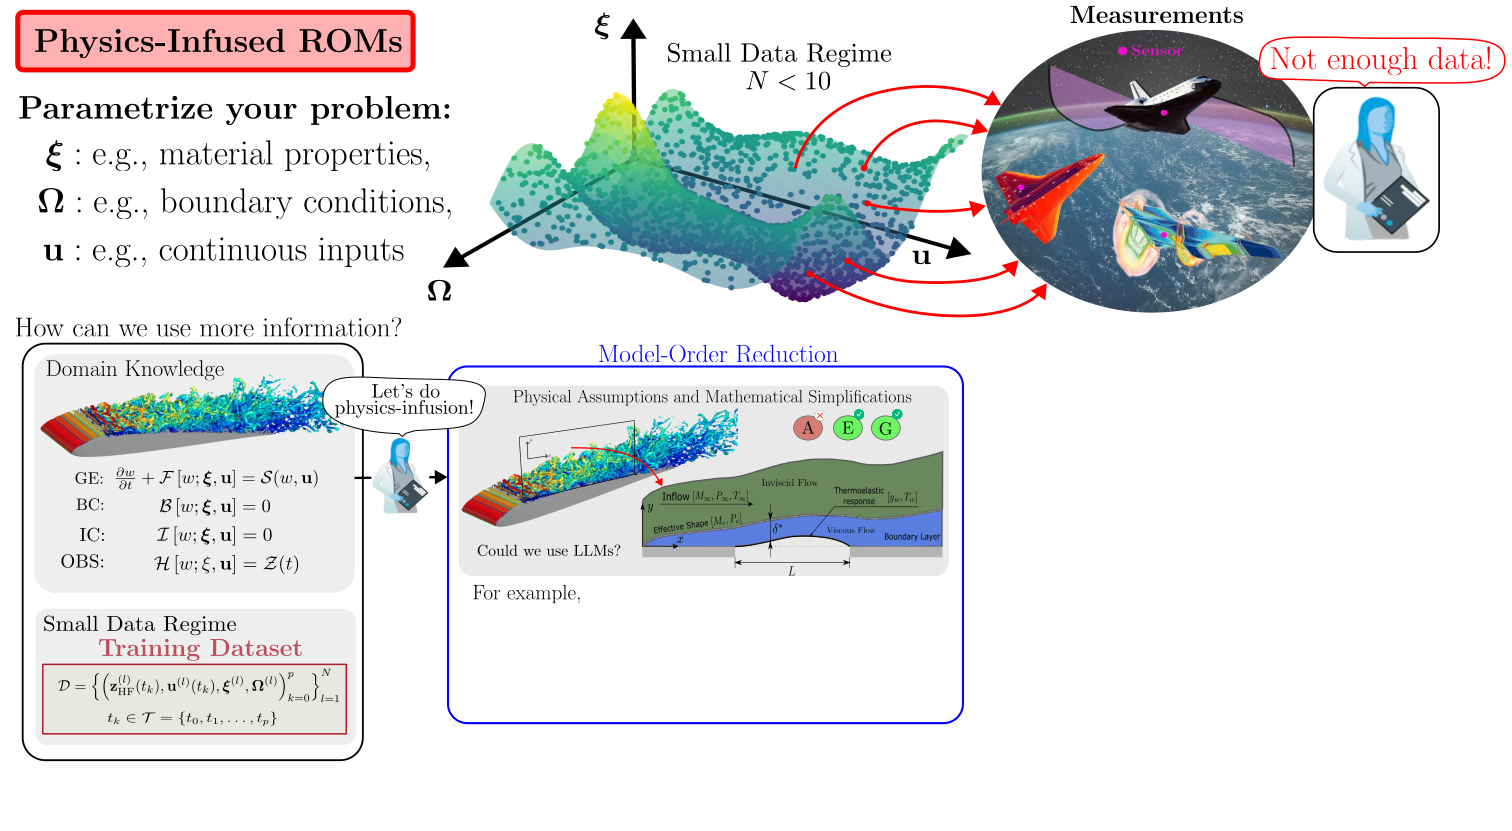
\includegraphics[width=0.9\textwidth]{../figs/sota/physics_infused_9.png}
    \end{figure}}
    \only<10>{
    \begin{figure}
        \centering
        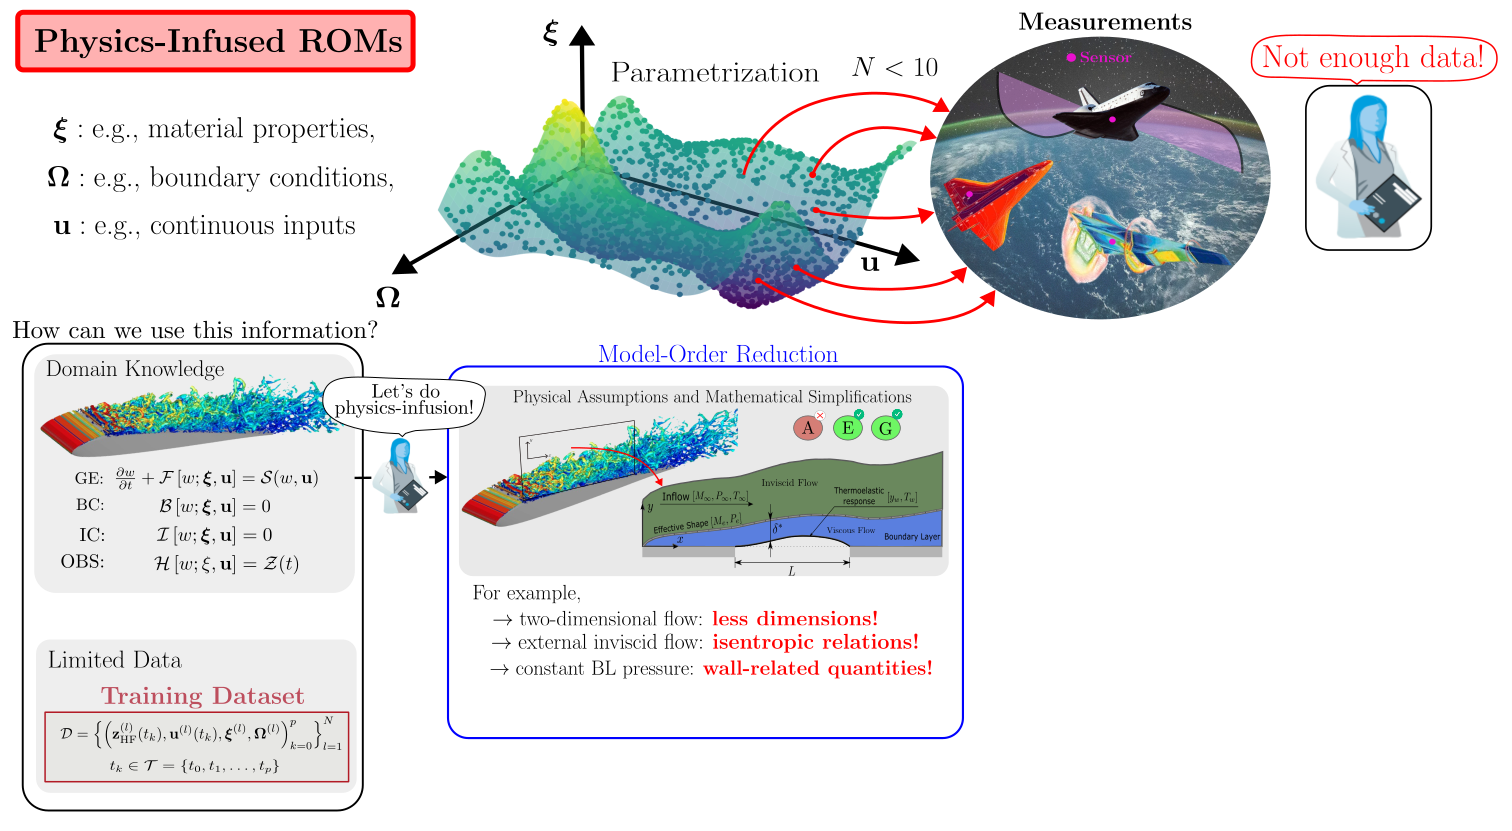
\includegraphics[width=0.9\textwidth]{../figs/sota/physics_infused_10.png}
    \end{figure}}
    \only<11>{
    \begin{figure}
        \centering
        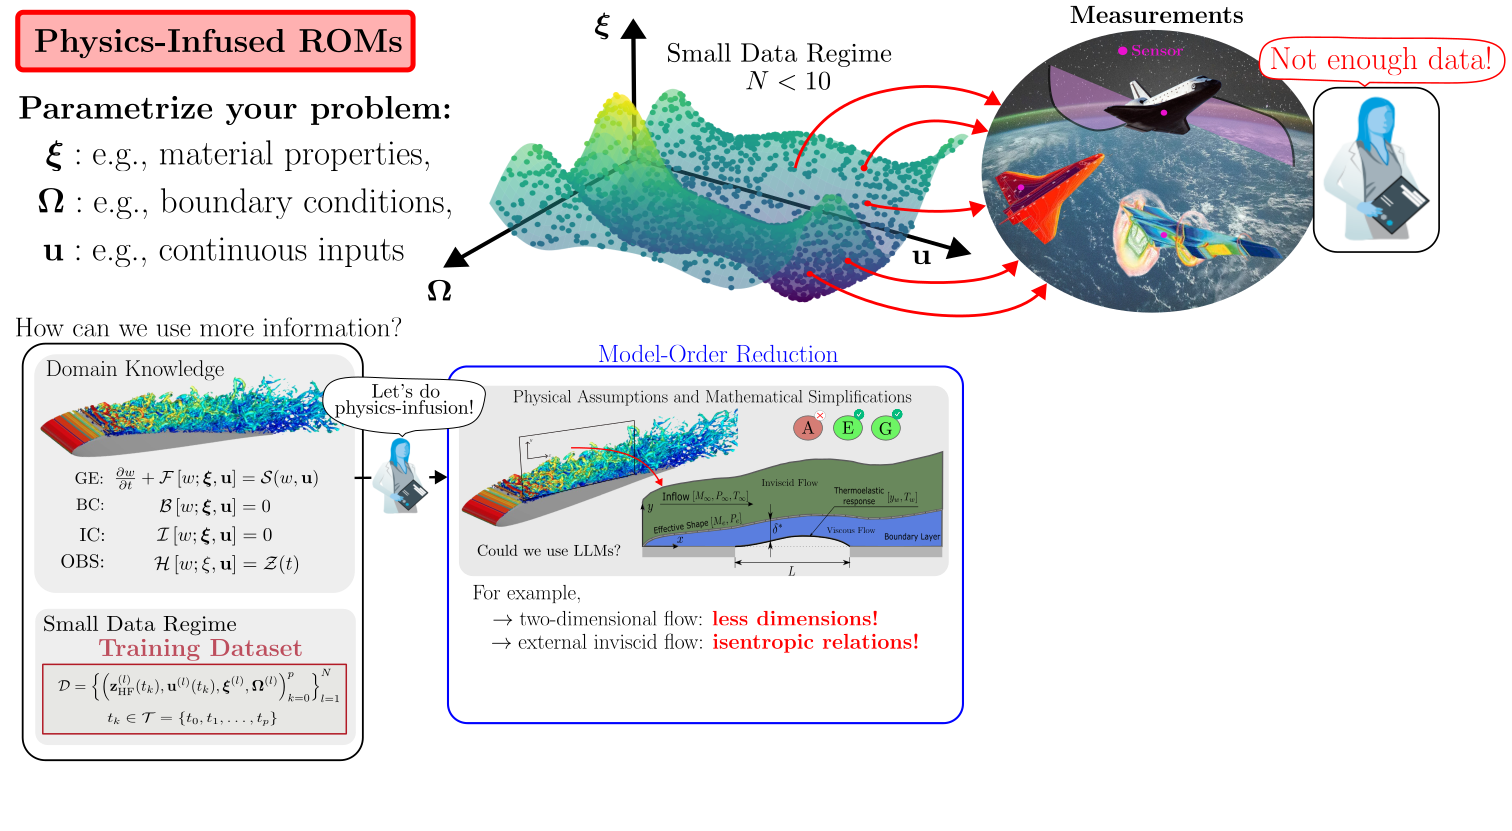
\includegraphics[width=0.9\textwidth]{../figs/sota/physics_infused_11.png}
    \end{figure}}
    \only<12>{
    \begin{figure}
        \centering
        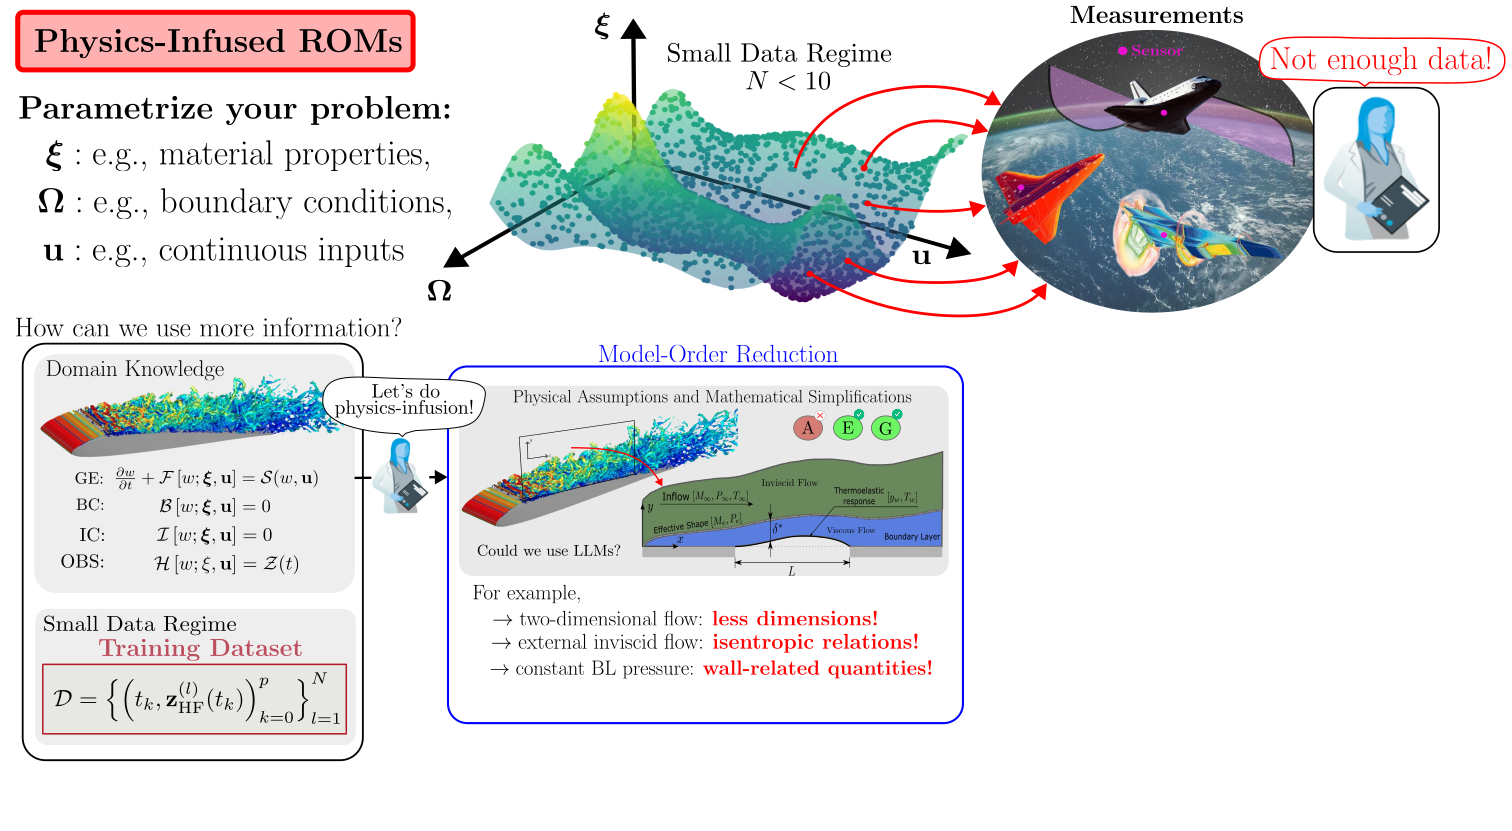
\includegraphics[width=0.9\textwidth]{../figs/sota/physics_infused_12.png}
    \end{figure}}
    \only<13>{
    \begin{figure}
        \centering
        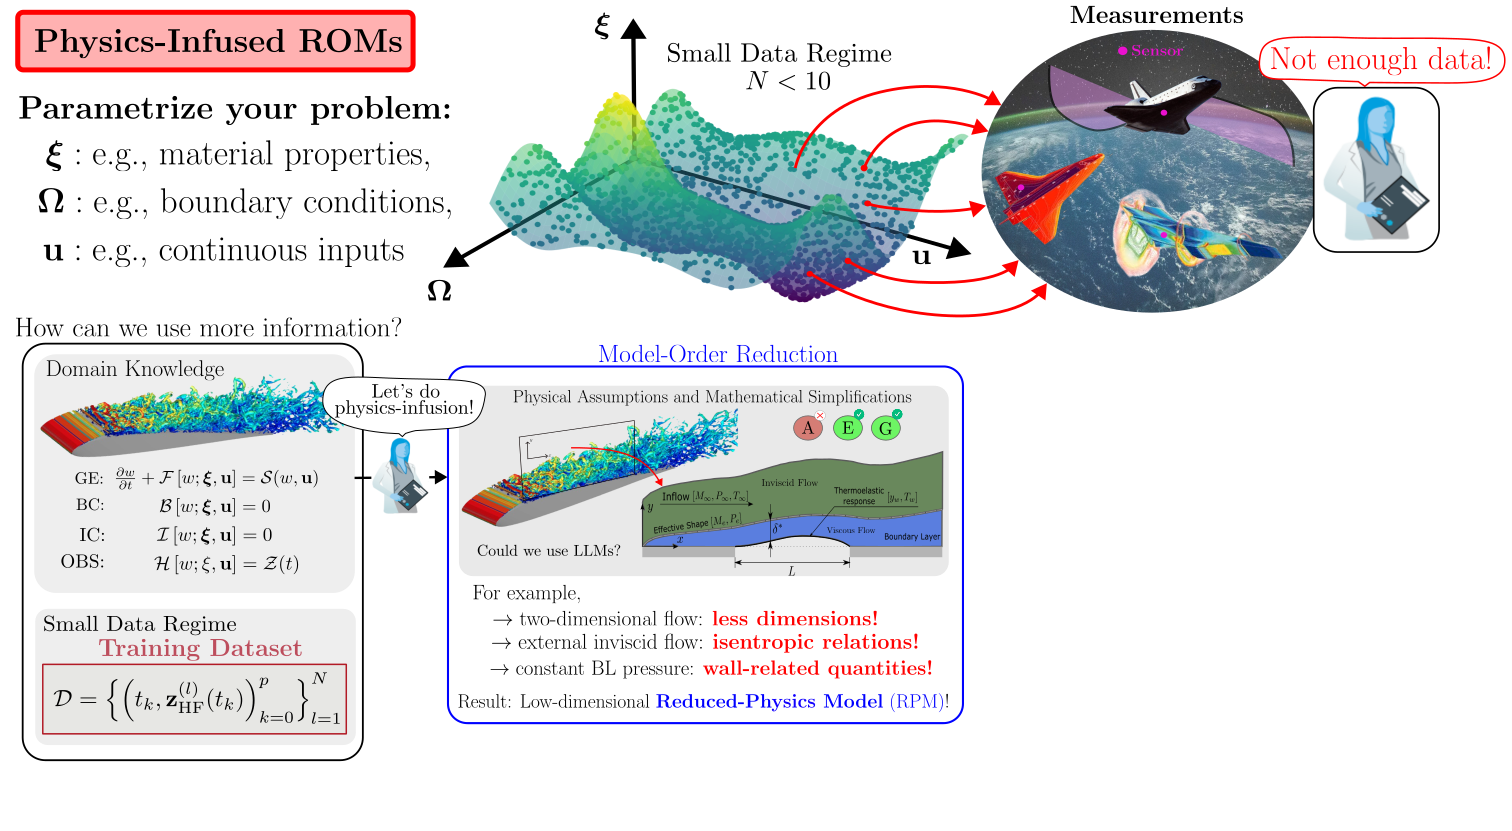
\includegraphics[width=0.9\textwidth]{../figs/sota/physics_infused_13.png}
    \end{figure}}
    \only<14>{
    \begin{figure}
        \centering
        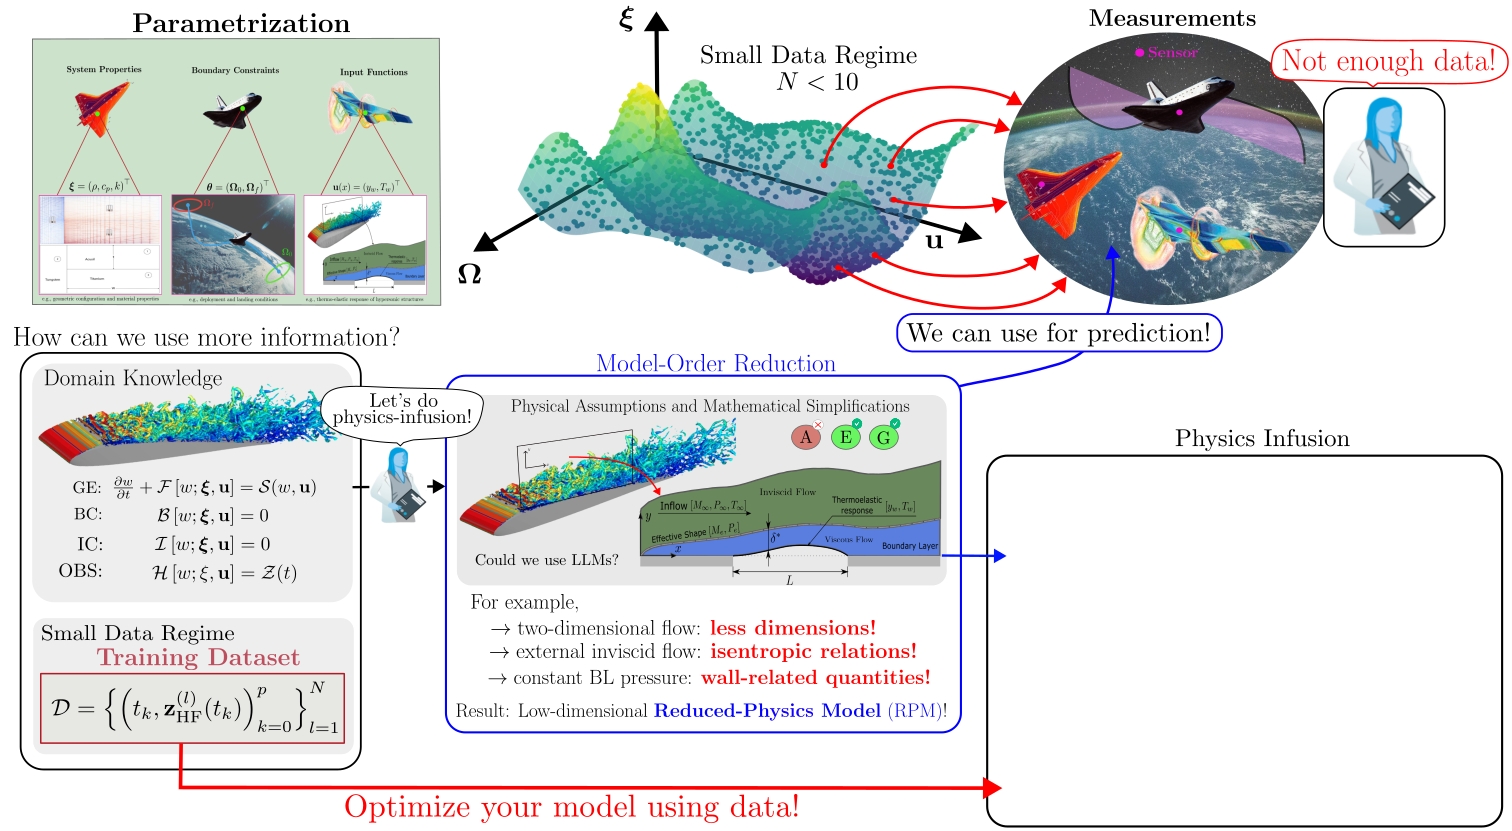
\includegraphics[width=0.9\textwidth]{../figs/sota/physics_infused_14.png}
    \end{figure}}
    \only<15>{
    \begin{figure}
        \centering
        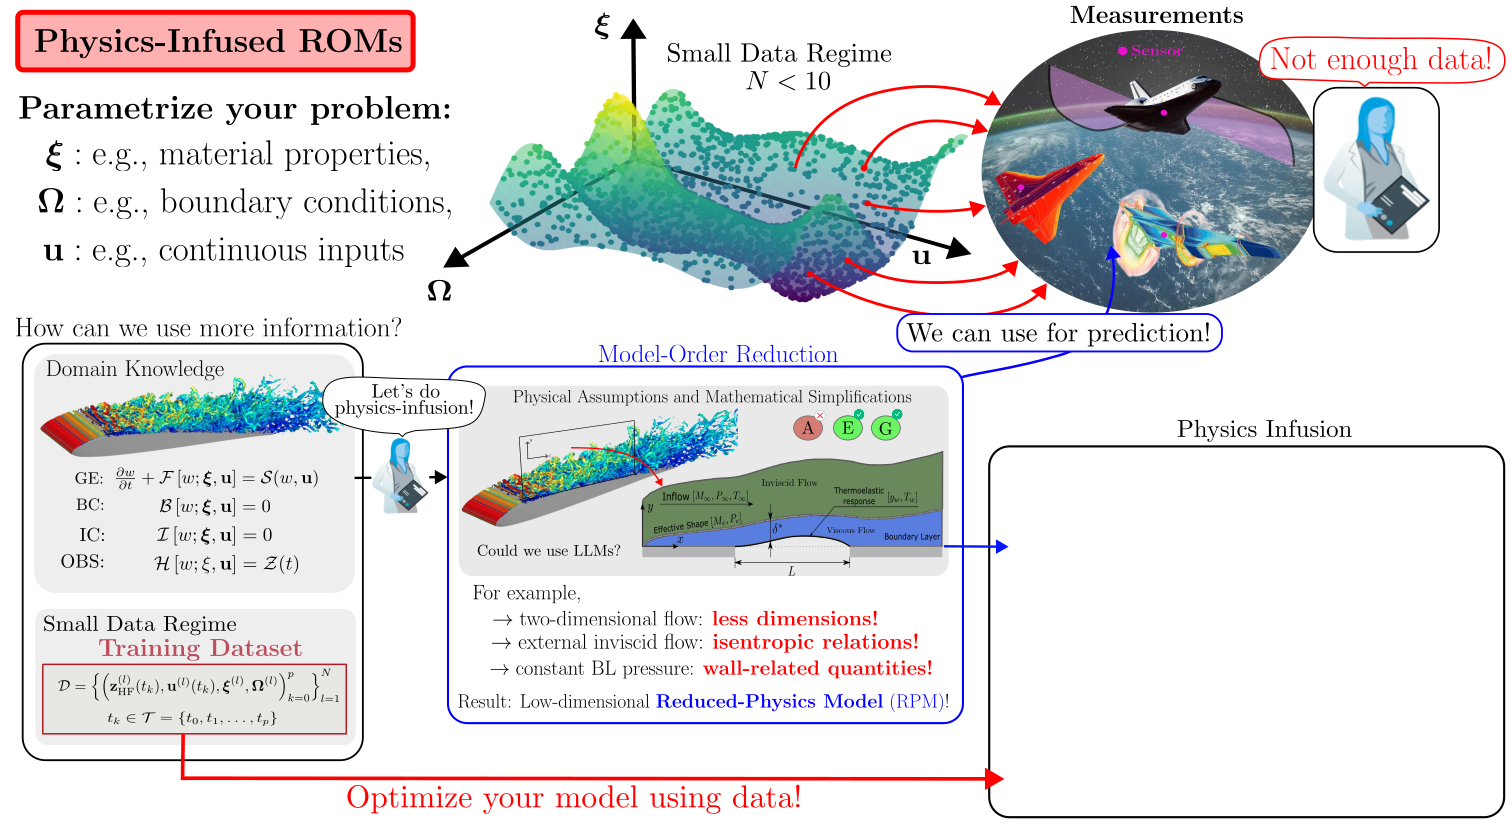
\includegraphics[width=0.9\textwidth]{../figs/sota/physics_infused_15.png}
    \end{figure}}
    \only<16>{
    \begin{figure}
        \centering
        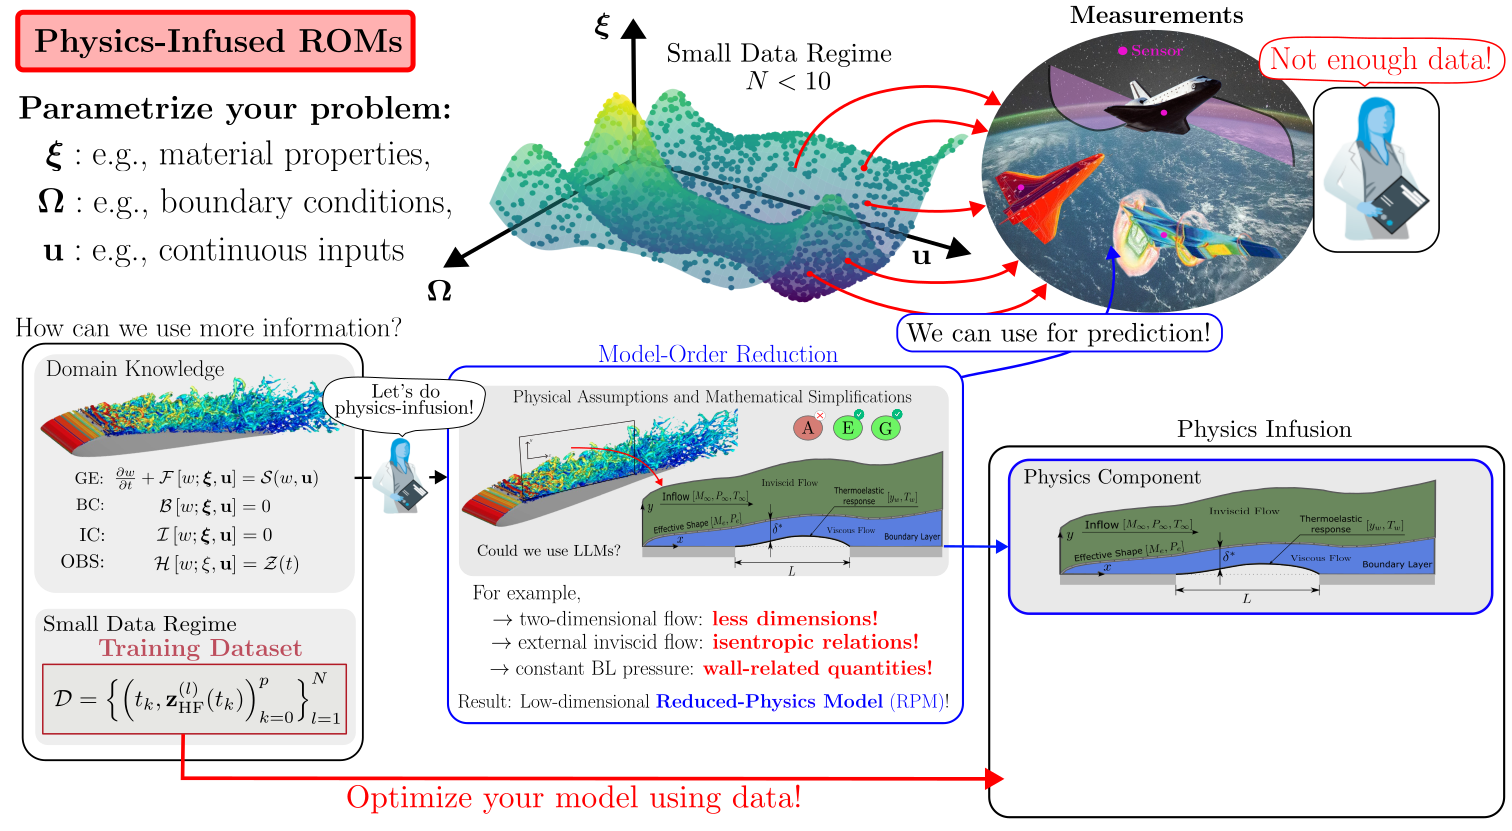
\includegraphics[width=0.9\textwidth]{../figs/sota/physics_infused_16.png}
    \end{figure}}
    \only<17>{
    \begin{figure}
        \centering
        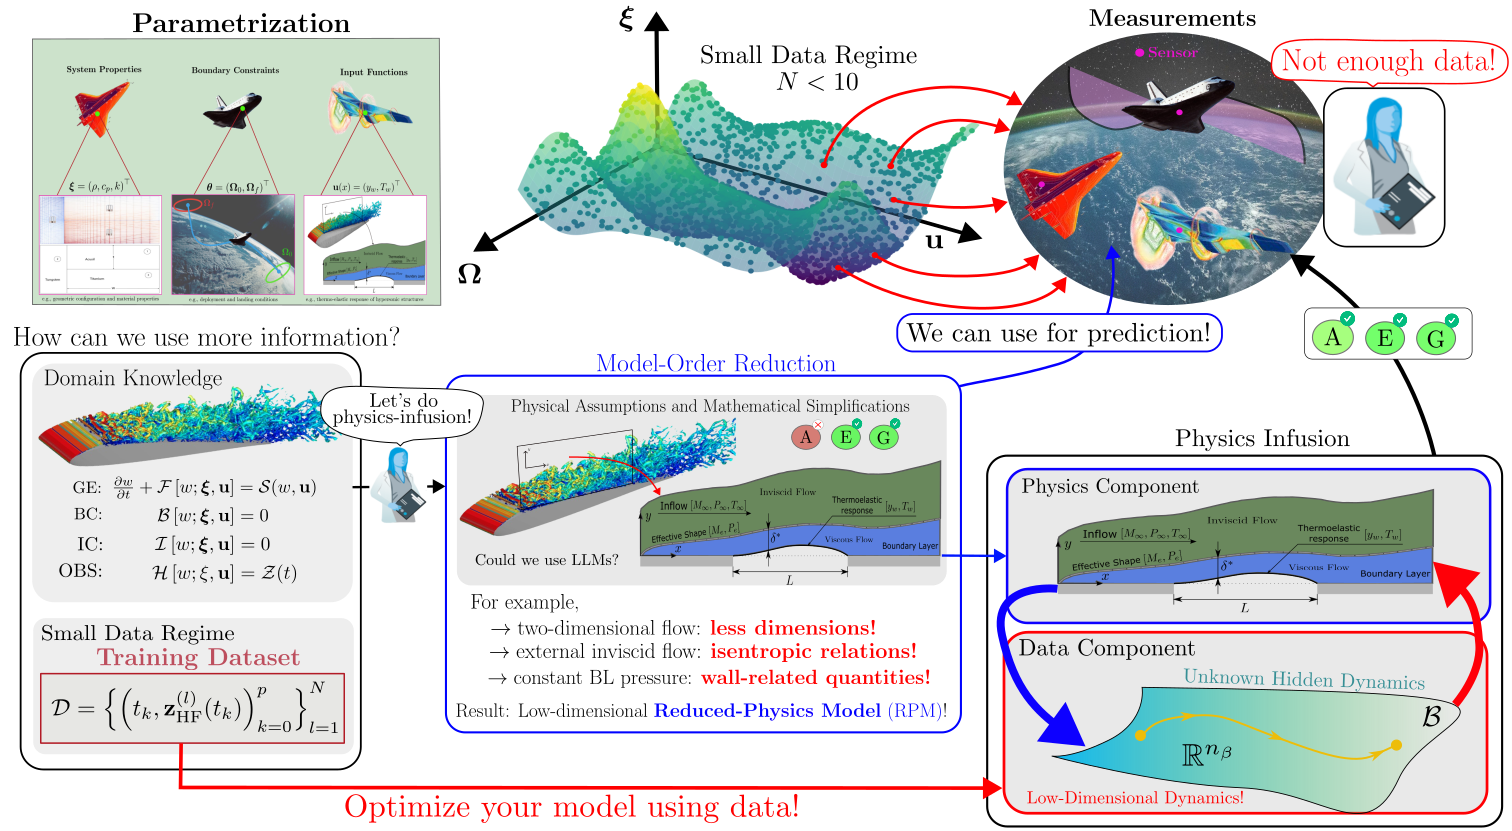
\includegraphics[width=0.9\textwidth]{../figs/sota/physics_infused_17.png}
    \end{figure}}
\end{frame}